\chapter{Boolean Formulas and Equations}
\label{ch:Boolean-Formulas}

\section{Reasoning with Equations}
\label{sec:math-and-equations}
\index{symbolic logic}\index{logic!symbolic}Symbolic logic,
like other parts of mathematics, starts from a small
collection of axioms and employs rules of inference to find
additional propositions consistent with those axioms. This
chapter will define a grammar of logic formulas, postulate a few
equations stating that certain formulas carry the same meaning as others,
and derive new equations
using substitution of equals for equals as the rule of
inference.

You will probably find this familiar from your
experience with numeric algebra, but the discourse here will attend carefully
to details, and this formality may extend beyond what you are
accustomed to. What it buys is mechanization. That is,
logic formulas and reasoning about them will amount to
mechanized computation, and this will make it possible for
computers to check that our reasoning follows all the rules,
without exception. This justifies more confidence
in conclusions than would otherwise be possible.

We will be doing all of this in the domain of symbolic logic, which
includes operations like ``logical or'' and ``logical negation'',
rather than arithmetic operations, such as addition and
multiplication.
We will be doing Boolean algebra, rather than numeric algebra,
but the underlying rule of inference, namely
substitution\index{reasoning!with equations}\index{substitution}\index{formula!substitution}
of equals for equals,
applies equally well to both Boolean and numeric formulas.
To illustrate the level of formality that we are shooting for,
let's see how it works with a problem
in the familiar domain of numeric algebra.

You are surely familiar with the equation $(-1)\times(-1) = 1$, but you may
not know that it is a consequence of some basic facts about
arithmetic.
That is, the fact that multiplying two
negative numbers produces a positive one
is not independent of other facts about numbers,
and it is not an arbitrary decision, either.
Instead, it is an inference one can draw
from an acceptance of other familiar equations.
We will derive the equation $(-1)\times(-1) = 1$
from equations that you have accepted without question for a long time.

The equations in Figure~\ref{fig-02-01} (page \pageref{fig-02-01})
express some standard rules of numeric computation.
In those equations, the letters stand in
place of numbers. They can also stand in place of other
formulas.
So, the variable $x$ stands for a grammatically correct formula,
which could be something simple, such as ``$2$'',
it could be a more complicated formula, such as ``$3\times(y + 1)$''.

We refer to letters used in this way as
\index{variable}variables even though, within a particular equation, they
stand for a fixed number or a particular formula.
The formula associated with a variable, though unspecified,
is the same for every occurrence of the variable in the equation.
If $x$ stands for $3\times(y + 1)$ at one point in the
equation, then everywhere else $x$ occurs in the equation,
it stands for that same formula, $3\times(y + 1)$.
This is the usual custom in algebra.

\begin{aside}{aside-hold-on-to-seat}{Hold on to Your Seat}
Mathematical formulas communicate
information using a formal grammar imbued with specific meanings.
The grammar determines which phrases are well formed
and which are not.
For example, ``$x+3\times(y + z)$'' conforms to a grammar
of numeric formulas.
It is grammatically correct, and it stands for a
particular and carefully prescribed calculation.
The non-formula ``$x+3\times(y + ) \times z$''
does not conform to that grammar and, therefore,
carries no meaning.
Reasoning about computer hardware and software
calls for a high degree of \index{formalism}formality to ensure
a level of consistency that is essential to  its usefulness.

Rigorous formality takes many readers by surprise.
It takes some getting used to.
Things may seem overly simple in the beginning.
Then, suddenly, you may find yourself thrashing around in deep water.
Take a deep breath, and slowly work  through the material.
It provides a basis for everything to follow.
The ideas and methods call for careful study and frequent review.
When things start to go off track,
slow down, back up a little, and try
again.\index{panic, don't}\index{disheartened?}\index{frustrated?}\index{baffled?}\index{worried?}\index{scared?}\index{funk, in a?}
Gradually, the pieces will fall into place,
but you can expect to run into some bumps.
\emph{Hold on to your seat.}
%\caption{Hold on to Your Seat}
%\label{aside-hold-on-to-seat}\index{seat, hold on}\index{hold onto your seat}
\end{aside}

\begin{figure}
\begin{center}
\begin{spacing}{0.9}
\begin{tabular}{ll}
$x+0 = x$                 & \{$+$ identity\} \\
$(-x)+ x = 0$             & \{$+$ complement\} \\
$x \times 1 = x$          & \{$\times$ identity\} \\
$x \times 0 = 0$          & \{$\times$ null\} \\
$x+y = y+x$               & \{$+$ commutative\} \\
$x \times y = y \times x$ & \{$\times$ commutative\} \\
$x+(y+z) = (x+y)+z$       & \{$+$ associative\} \\
$x \times (y \times z) = (x \times y) \times z$ & \{$\times$ associative\} \\
$x\times(y+z) = (x \times y)+(x \times z)$      & \{distributive law\} \\
\end{tabular}
\end{spacing}
\end{center}\index{equation, by name!\{$+$ identity\}}\index{equation, by name!\{$+$ complement\}}\index{equation, by name!\{$\times$ identity\}}\index{equation, by name!\{$\times$ null\}}\index{equation, by name!\{$+$ commutative\}}\index{equation, by name!\{$\times$ commutative\}}\index{equation, by name!\{$+$ associative\}}\index{equation!numeric algebra}\index{axiom!numeric algebra}\index{reasoning!with equations}
\caption{Equations of Numeric Algebra}
\label{fig-02-01}
\end{figure}

If we accept the equations of Figure~\ref{fig-02-01},
we can apply one of them to transform the formula $(-1)\times(-1)$ to a new formula that
stands for the same number. Then, we can apply another equation to
transform that formula to a new one, and so on.
We look for a way to apply the
accepted equations one by one, so that in the end we
arrive at the formula ``1''. At every step, we know that the
new formula stands for the same number as the old one, so in
the end we know that $(-1)\times(-1) = 1$.

Figure~\ref{fig-02-02} (page \pageref{fig-02-02})
displays this sort of equation-by-equation derivation of the
formula ``1'' from the formula ``$(-1)\times(-1)$''. To
understand Figure~\ref{fig-02-02}, you must remember that each
variable can denote any
grammatically correct formula. For example, in the
equation, $x + 0 = x$,
which is called the \{$+$ identity\} equation,
the variable $x$ could stand for a number,
such as 3, or it could stand for a more complicated
formula, such as $(1 + 3)$. It could even stand for a formula
with variables in it, such as $(a + (b \times c))$ or
$(((-1) \times (x + 3)) + (x + y))$.

Another crucial point is that each step cites
exactly one equation from Figure~\ref{fig-02-01}
to justify the transformation from the formula in the previous step.
We are so accustomed to calculating with numeric formulas that
we often combine many basic steps into one. When we reason formally,
we are careful to do just one step at a time.
We justify each step by citing an equation
from a list of known equations. In our proof of $(-1)\times(-1) = 1$,
we will justify steps by citing equations from Figure~\ref{fig-02-01}
and from no other source. We will not skip steps.
Keep that in mind as you go through the proof, line by line.

The first step in the proof
(Figure~\ref{fig-02-02}, page \pageref{fig-02-02}) uses a version of the
\{$+$ identity\} equation in which the variable $x$ stands for the
formula $((-1)\times(-1))$.
In this context, the \{$+$ identity\} equation
leads to the new formula $((-1)\times(-1)) + 0$.

The second step in the proof reads the \{$+$ complement\}
equation backwards (equations go both ways), and in a form
where the variable $x$ stands for the number 1.
When $x$ is 1, the \{$+$ complement\} equation is
$(-1) + 1 = 0$.
Reading the equation backwards, we can substitute
$((-1) + 1)$ for $0$,
and that leads to the formula $((-1)\times(-1)) + ((-1) + 1)$.
So, we know now that
$(-1)\times(-1) = ((-1)\times(-1)) + ((-1) + 1)$.

Doesn't really seem like progress does it?
But, we press on anyway, one step at a time.
The transformations, step by step, finally confirm that the two formulas
$(-1)\times(-1)$ and 1 represent the same number.

Pay particular attention to the last three lines of the proof.
Most people tend to jump from the formula $0+1$ to the
formula $1$ in one step. That jump requires knowing the equation
$0+1 = 1$. However, that equation is not among those listed in
Figure~\ref{fig-02-01}.
We want to do the proof without citing any equations
other than those in Figure~\ref{fig-02-01}, so we need two steps
to get from ``$(0+1)$'' to ``$1$'',
and those are the last two steps in the proof.

\begin{figure}
\begin{center}
\begin{spacing}{0.9}
\begin{tabular}{lll}
    & $(-1)\times(-1)$                            & \\
$=$ & $((-1)\times(-1)) + 0$                      & \{$+$ identity\} \\
$=$ & $((-1)\times(-1)) + ((-1) + 1)$             & \{$+$ complement\} \\
$=$ & $(((-1)\times(-1)) + (-1)) + 1$             & \{$+$ associative\} \\
$=$ & $(((-1)\times(-1)) + ((-1) \times 1)) + 1$  & \{$\times$ identity\} \\
$=$ & $((-1)\times((-1) + 1)) + 1$                & \{distributive law\} \\
$=$ & $((-1)\times 0) + 1$                        & \{$+$ complement\} \\
$=$ & $0 + 1$                                     & \{$\times$ null\} \\
$=$ & $1 + 0$                                     & \{$+$ commutative\} \\
$=$ & $1$                                         & \{$+$ identity\} \\
\end{tabular}
\end{spacing}
\end{center}\index{negative $\times$ negative}\index{equation!proof by}\index{proof!with equations}\index{commutative}\index{distributive}\index{reasoning!with equations}\index{equation!citation}\index{citation!equation}
\caption{Why $(-1)\times(-1)=1$}
\label{fig-02-02}
\end{figure}

One of the things we hope you will glean from this derivation is that
the equation $(-1)\times(-1) = 1$ does not depend on vague,
philosophical assertions like ``two negatives make a positive.''
Instead, the equation $(-1)\times(-1) = 1$ is a consequence of some
basic arithmetic equations. If you accept the basic equations
and the idea of substituting equals for equals,\footnote{Substituting
equals for equals applies the first of
\index{Euclid}Euclid's \index{common notions}common notions:
Things which are equal to the same thing are also equal to one another.
%Failed attempt to quote Euclid in Greek ... probably bad idea anyway
%(Or, ``\textgreek{Ηἰτήσθω ἀπὸ παντὸς σημείου ἐπὶ πᾶν σημεῖον εὐθεῖαν γραμμὴν ἀγαγεῖν}'',
%as Euclid may have put it.)
People have been reasoning by substitution for a long time.}
you must, as a rational consequence, accept the equation
$(-1)\times(-1) = 1$.

Using this same kind of reasoning, we will derive new Boolean equations
from a few, basic ones postulated as axioms.
A Boolean \emph{axiom} is a Boolean equation
that we assume to be true, without proof.
We will also learn that digital circuits are physical
manifestations of logic formulas, and we will be able to
parlay that idea to derive behavioral properties of
computer components.

Likewise, because a computer program is,
literally, a formula, we will be able to derive
properties of software directly from the programs, themselves.
This makes it possible for us to be entirely
certain about some of the behavioral characteristics of
software and of the digital circuits that
comprise hardware components.
Our certainty stems from the mechanistic
\index{formalism}formalism that we insist on from the beginning,
which can be checked to the last detail with automated computation.

\begin{exercises}
\label{ex:ch02-intro}
\exer {Use the equations of Figure~\ref{fig-02-01} (page \pageref{fig-02-01}),
together with the additional equation (1+1)=2, to derive the equation $(x + x) = (2 \times x)$.}

\exer {\label{ex:times-negation}%
Derive the following equation
using using the equations of Figure~\ref{fig-02-01}.
\begin{center}
$((-1) \times x) + x = 0$ ~~~~~ \{$\times$ negation\}
\end{center}}

\exer {Derive the equation $((x + (((-1) \times (x + y)) + z)) + y) = z$
using using the equations of Figure~\ref{fig-02-01} and,
if you like,
the \{$\times$ negation\} equation from Exercise \ref{ex:times-negation}.}
\end{exercises}

\section{Boolean equations}
\label{sec:boolean-equations}
Let's start with the Boolean equations in
Figure~\ref{fig-02-03} (page \pageref{fig-02-03}).
These equations, which we will call the
\index{Boolean!axiom}Boolean \index{axiom!Boolean algebra}axioms,
are the starting point for our system of reasoning.
They form the basis from which we will derive
a host of other equations.
If these axiomatic \index{equation!as axiom}equations
are new to you and seem strange,
try to view them as ordinary,
algebraic equations, but with a different collection of operators.
A formula in numeric algebra has operations like addition
($+$) and multiplication ($\times$). Boolean formulas employ logic
operations: logical-and ($\wedge$), logical-or ($\vee$),
logical-negation ($\neg$), and implication ($\rightarrow$).
Furthermore, Boolean formulas stand for logic values
($True$, $False$), rather than for numbers (\dots -2, -1, 0, 1, 2 \dots).

\begin{figure}
\begin{center}
\begin{spacing}{0.9}
\begin{tabular}{ll}
$x \vee False = x$                                   & \{$\vee$ identity\} \\
$x \vee True = True$                                 & \{$\vee$ null\} \\
$x \vee y = y \vee x$                                & \{$\vee$ commutative\} \\
$x \vee (y \vee z) = (x \vee y) \vee z$              & \{$\vee$ associative\} \\
$x \vee (y \wedge z) = (x \vee y) \wedge (x \vee z)$ & \{$\vee$ distributive\} \\
$x \rightarrow y = (\neg x) \vee y$                  & \{implication\} \\
$\neg(x \vee y) = (\neg x) \wedge (\neg y)$          & \{$\vee$ DeMorgan\} \\
$x \vee x = x$                                       & \{$\vee$ idempotent\} \\
$x \rightarrow x = True$                             & \{self-implication\} \\
$\neg(\neg x)  = x$                                  & \{double negation\} \\
\end{tabular}
\end{spacing}
\end{center}\index{Boolean!algebra}\index{commutative}\index{distributive}\seeonlyindex{algebra, Boolean}{Boolean, algebra}\index{reasoning!with equations}\index{axiom!commutative}\index{axiom!associative}\index{axiom!parentheses}\index{axiom!Boolean algebra}\index{axiom, by name!\{$\vee$ identity\}}\index{axiom, by name!\{$\vee$ null\}}\index{axiom, by name!\{$\vee$ commutative\}}\index{axiom, by name!\{$\vee$ associative\}}\index{axiom, by name!\{$\vee$ distributive\}}\index{axiom, by name!\{implication\}}\index{axiom, by name!\{$\vee$ DeMorgan\}}\index{axiom!DeMorgan}\index{axiom, by name!\{$\vee$ idempotent\}}\index{axiom!idempotent}\index{axiom, by name!\{self-implication\}}\index{axiom, by name!\{double negation\}}\index{axiom, by name!\{atomic release\}}\index{equation!grammar}\index{equation!distributive}\index{equation!Boolean algebra}\index{equation!commutative}\index{equation!associative}\index{equation!parentheses}\index{equation!Boolean algebra}\index{equation, by name!\{$\vee$ identity\}}\index{equation, by name!\{$\vee$ null\}}\index{equation, by name!\{$\vee$ commutative\}}\index{equation, by name!\{$\vee$ associative\}}\index{equation, by name!\{$\vee$ distributive\}}\index{equation, by name!\{implication\}}\index{equation, by name!\{$\vee$ DeMorgan\}}\index{equation!DeMorgan}\index{equation, by name!\{$\vee$ idempotent\}}\index{equation, by name!\{idempotent\}}\index{equation, by name!\{self-implication\}}\index{equation, by name!\{double negation\}}\index{operator, logic!and ($\wedge$)}\index{operator, logic!or ($\vee$)}\index{operator, logic!not ($\neg$)}\index{operator, logic!implication ($\rightarrow$)}\seeonlyindex{logic operator}{operator, logic}
\caption{Boolean Axioms (basic equations)}
\label{fig-02-03}
\end{figure}

When we derive a new equation by citing an equation that was,
itself, derived, rather than by citing an axiomatic equation
from Figure~\ref{fig-02-03},
we refer to the cited equation as a \index{theorem}\emph{theorem} to
distinguish it from an axiom.
The new \index{equation!as theorem}equation is also a theorem,
and it can be cited in \index{derivation}derivations of other new equations.
We call such a derivation of a new equation a
\index{proof}\emph{proof} of the equation.

\begin{figure}
\begin{theorem}[\{$\vee$ truth table\}]
\mbox{}
\begin{itemize}
\item $False \vee False = False$
\item $False \vee True  = True$
\item $True  \vee False = True$
\item $True  \vee True  = True$
\end{itemize}
\end{theorem}

\begin{proof}
\mbox{}\\
\begin{tabular}{llll}
    &$False \vee False$    & \\
$=$ & $False$              & \{$\vee$ identity\}  &---replace $x$ in the axiom with \emph{False}\\
    &  ~                   & \\
    & $False \vee True$    & \\
$=$ & $True$               & \{$\vee$ null\}      &---replace $x$ in the axiom with \emph{False}\\
%    &                      & \dots for practice, prove the other two equations yourself \dots \\
\end{tabular}
\begin{quote}
\dots for practice, prove the other two equations yourself \dots
\end{quote}
\end{proof}
\index{equation!proof by}
\index{proof!with equations}
\index{truth table}
\caption{Proof of Theorem \{$\vee$ Truth Table\}}
\label{or-truth-table}
\end{figure}

The first equation in the theorem \{$\vee$ truth table\}
(Figure~\ref{or-truth-table}, page \pageref{or-truth-table})
is a special case of the
\{$\vee$ identity\} axiom (Figure~\ref{fig-02-03}),
and the proof of that equation simply amounts making that observation.
That is, the proof just rewrites the \{$\vee$ identity\} axiom
with $False$ in place of $x$.
The proof of the second equation is equally short, but cites
a different axiom.
For practice, try to prove the other two
equations in the \{$\vee$ truth table\} theorem
by citing axioms in a similar way.

We are serious about that. Did you prove the other two equations?
No? Well \dots go back and do it, then. Without participation, there
is no learning. $\dots$ \emph{We'll wait here}$\dots$

Finished now? Good for you. You cited the \{$\vee$ identity\} axiom in your
proof of the third equation in the theorem and the \{$\vee$ null\}
axiom in your proof of the fourth equation, right? We knew you could do it.

\begin{aside}{truth-tables}{Truth Tables}
A \emph{truth table} for a formula is a list of equations
stating the values that the formula represents.
There is one equation in the truth table for each possible
combination of values for the variables in the formula.
If there is only one variable in the formula,
there will be two equations in its truth table,
one for the case when the variable has the value
$True$ and one for the case when it has the value $False$.
If there are two variables in the formula,
there will be four equations in the truth table
because for each choice of value for the first variable,
there are two choices for the other.
Three variables lead to eight equations.
The number of equations in the truth table
doubles with each additional variable
in the formula.

A truth table for a logic operator is the truth table for the formula
that has variables in place of the operands.
For example, the truth table for the logical-or operator ($\vee$)
is the truth table for the formula $(x \vee y)$.
That formula has two variables, so the truth table has four equations.
%\caption{Truth Tables}
%\label{truth-tables}
\end{aside}

Derivations are usually more than one step, of course.
The \{$\vee$ complement\} theorem
(Figure~\ref{fig:or-complement-thm}, page \pageref{fig:or-complement-thm})
has a two-step proof, citing the \{implication\} axiom
and the \{self-implication\} axiom.
The \{$\vee$ complement\} theorem is often called the
\index{law of the excluded middle}``law of the excluded middle''
because it says that any logic formula,
together with its negation, covers all of the possibilities.
A formula in logic is either true of false.
There is no middle ground.

\begin{figure}
\begin{theorem}[\{$\vee$ complement\}]
$(\neg x) \vee x = True$
\end{theorem}
\begin{proof}
\mbox{}\\
\begin{tabular}{lll}
    & $(\neg x) \vee x$ & \\
$=$ & $x \rightarrow x$ & \{implication\} \\
$=$ & $True$            & \{self-implication\} \\
\end{tabular}

\end{proof}
\index{equation!proof by}
\index{proof!with equations}
\index{equation, by name!\{$\vee$ complement\}}
\index{excluded middle}
\index{equation!excluded middle}
\index{law of the excluded middle}
\caption{Proof of Theorem \{$\vee$ complement\}}
\label{fig:or-complement-thm}
\end{figure}

All of the logic operators have truth tables,
and we can derive the equations in those truth tables from the axioms.
Figure~\ref{fig:neg-truth-table} (page \pageref{fig:neg-truth-table})
displays the truth table
for the negation operator $(\neg)$.
The figure includes a four-step proof of the first equation in
the table.
To beef up your comprehension of the ideas,
construct your own proof of the second equation in the theorem.

\begin{figure}
\begin{theorem}[\{$\neg$ truth table\}]
\mbox{}\\
\begin{itemize}
\item $\neg True = False$
\item $\neg False = True$
\end{itemize}
\end{theorem}
\begin{proof}
\mbox{} \\
\begin{tabular}{llll}
    & $\neg True$                      & \\
$=$ & $\neg (False \rightarrow False)$ & \{self-implication\} \\
$=$ & $\neg ((\neg False) \vee False)$ & \{implication\}     &---replace $x$ and $y$ in axiom with $False$ \\
$=$ & $\neg (\neg False)$              & \{$\vee$ identity\} &---replace $x$ in the axiom with $\neg False$ \\
$=$ & $False$                          & \{double negation\} &---replace $x$ in axiom with $False$ \\
\end{tabular}

\bigskip
\noindent
\begin{tabular}{lll}
    & $\neg False$                             & \\
$=$ & \dots you fill in the details here \dots & \\
$=$ & $True$                                   & \\
\end{tabular}

\end{proof}
\index{equation!proof by}
\index{proof!with equations}
\index{truth table}
\caption{Proof of Theorem \{$\neg$ truth table\}}
\label{fig:neg-truth-table}
\end{figure}

An important facet of these proofs is that they are
entirely syntactic. That is, they apply axioms by
matching the grammar of a formula $f$ (or a sub-formula of $f$) in the proof
with a formula $g$ from one side of an equation in the axioms.
The matching associates the variables in $g$ with corresponding sub-formulas of $f$.
Then, the formula $h$ on the other side of
the axiomatic equation is rewritten,
replacing each variable in $h$ with the subformula of $f$
that the matching process established.
The rewritten version of $h$
becomes the new, derived formula.
We know that the derived formula stands for the same value
as the original formula because the axiom asserts this equivalence,
and we assume the axioms are right.

\begin{aside}{feasibility}{Truth Tables and Feasibility}
Reasoning from equations is one way to prove that two formulas stand
for the same value.
Another way is to build truth tables for both formulas.
If the tables match, value for value, you can conclude that
the formulas are equal.
When there are only a few variables, and therefore only a few combinations,
the truth tables can be compared quickly and accurately.
Unfortunately, this approach quickly goes south when there are many variables.
With two variables, as in the truth table
for logical-or, there are four combinations of values
(two choices for each variable, $True$ or $False$, so two times two
combinations in all). With three variables, there are eight
($2^3$) combinations, which makes the truth-table method tedious,
but not infeasible.

With ten variables, there are 1,024 ($2^{10}$) combinations,
and with twenty, over a million.
Too much for people to handle, but easy for computers.
However, a formula specifying a computing component,
hardware or software, has hundreds of variables.
We want to reason about computing components,
and there is no hope of doing that with truth tables.
With a hundred variables, there are $2^{100}$ combinations,
and that number is so large that no computer could
finish checking all the cases before the sun runs out of fuel.
Truth tables are infeasible in this realm.

Proofs like those that make up the core of this book
are not the only effective way to work with large formulas.
Hardware and software designers sometimes use
SMT solvers (satisfiability modulo theories),
BDD tools (binary decision diagrams), or other similar methods
to verify properties of circuits and computer programs,
but such tools don't apply to all formulas.
Reasoning based on grammatical form
makes it feasible to deal with any logic formula,
regardless of the number of variables,
because the formulas can be split into parts small enough
to manage, and those parts can be reintegrated, based on
their grammatical relationships, to produce a full analysis.
Feasible doesn't mean easy, though.
It takes a lot of effort, but it can pay off.\index{truth table}\index{feasibility}\index{infeasibility}
%\caption{Truth Tables and Feasibility}
%\label{feasibility}
\end{aside}

Let's prove another truth-table theorem, partly to practice
reasoning with equations, but also to discuss a common
point of confusion about logic. The implication operator
($\rightarrow$) is a cornerstone of logic in real-world problems,
but it is common to get tripped up when it comes to
reasoning with implication.

The \{$\rightarrow$ truth table\} theorem
(Figure~\ref{implication-truth-table}, page \pageref{implication-truth-table})
provides the truth table
for the implication operator.
An important aspect of the proof is that it cites
not only axioms from Figure~\ref{fig-02-03} (page \pageref{fig-02-03}),
but also equations from the \{$\neg$ truth table\} theorem.
This is the way mathematics goes. Once we have derived
a new equation from the axioms, we can cite
the new equation to derive still more equations.

\begin{aside}{abstraction}{Abstraction}
Citing proven theorems to prove new ones
is similar to an idea known as
\index{abstraction}abstraction
in engineering design.
Instead of citing an old theorem to prove a new one,
we could copy the proof of the old theorem into the new proof.
However, that would make the proof longer, harder to understand,
and more likely to contain errors.

Computer programs are built from components that are, themselves,
also computer programs. As components become available,
they are used to build more complex components.
Sometimes, a component has almost the right form
to be used in a new program, but not quite.
Maybe the existing component doubles a number,
but the new usage needs to triple it.
It is tempting to copy the
old component, change $2 \times x$ to $3 \times x$,
and paste the revised component into the program.

In our experience, \index{copy-and-paste programming}copy-and-paste
programming is a common source of errors in software,
especially in programs maintained
over time. When a maintainer finds an error in
a component that was copied from elsewhere,
there is nothing to direct the maintainer to fix
the same error in the original component.
A better choice, most of the time,
is to make a new component with
a variable, say $m$, in place of the $2$.
This is known as creating an abstraction of the component
(``abstract'' as opposed to ``specific'' or ``concrete'').

The new component can be used for both doubling and tripling,
simply by specifying $2$ for $m$ in one case and $3$ for $m$ in the other.
If, later in the project, an error is discovered in the component,
the error only needs to be fixed in one place, not two,
or maybe ten or a hundred places, depending on how many engineers
copied the original component to make a change.
Abstraction is an important engineering method.
Citing old theorems to prove new ones has similar advantages.
%\caption{Abstraction}
%\label{abstraction}
\end{aside}

\begin{figure}
\begin{theorem}[\{$\rightarrow$ truth table\}]
\mbox{}
\begin{itemize}
\item $False \rightarrow False = True$
\item $False \rightarrow True  = True$
\item $True  \rightarrow False = False$
\item $True  \rightarrow True  = True$
\end{itemize}
\end{theorem}

\begin{proof}
\mbox{} \\
\begin{tabular}{llll}
    & $False \rightarrow False$        & \\
$=$ & $(\neg False) \vee False$        & \{implication\} &---\emph{put} $False$ \emph{for} $x$ \emph{and for} $y$ \emph{in axiom}\\
$=$ & $\neg False$                     & \{$\vee$ identity\}\\
$=$ & $True$                           & \{$\neg$ truth table\}\\
\end{tabular}

\begin{tabular}{lll}
& \dots for practice, prove the other equations yourself\dots & \\
\end{tabular}

\end{proof}
\caption{Proof of Theorem \{$\rightarrow$ truth table\}}
\index{truth table}
\label{implication-truth-table}
\end{figure}

In day-to-day life outside the domain of symbolic logic,
the usual interpretation of the logical implication ``$x \rightarrow y$''
is to conclude that $y$ is true if whenever
$x$ is true. However, the implication says nothing
about $y$ when $x$ is not true. In particular, it
does not say that $y$ is not true when $x$ is not true.
Theorem \{$\rightarrow$ truth table\} shows that the
formula ``$False \rightarrow y$'' has the value $True$ when $y$ is $True$
and also when $y$ is $False$.
In other words, the truth of the formula $x \rightarrow y$ in the case
where the operand on the left of the arrow (which is known as the
\index{discharge assumption}\index{Assume (natural deduction)!discharge}\index{hypothesis!discharge}\index{implication ($\rightarrow$)}\index{implication ($\rightarrow$)!hypothesis}\index{hypothesis!implication ($\rightarrow$)}\emph{hypothesis}
of the implication), $x$, is $False$ provides
no information about the right-hand operand, $y$ (which is known as the
\index{conclusion!implication ($\rightarrow$)}\index{implication ($\rightarrow$)!conclusion}\emph{conclusion}
of the implication).

A common mistake in everyday life is to infer from the truth of the
implication ``$x \rightarrow y$'' that the implication
``$(\neg x) \rightarrow (\neg y)$''
is also true. Sometimes this leads to bad
results, even in everyday life.\footnote{If turtles
are reported in the park,
you can conclude that there are reptiles in the park,
but if no turtles are reported, you cannot conclude
that there are no reptiles.
There might be rattlesnakes.
In the notation of logic,
\emph{turtle} $\rightarrow$ \emph{reptile} is true,
but ($\neg$\emph{turtle}) $\rightarrow$ ($\neg$\emph{reptile}) isn't.}
In symbolic logic,
it is worse than that. Such a conclusion puts an
inconsistency into the mathematical system, and that renders the system useless.

Over half of the Boolean axioms in Figure~\ref{fig-02-03} (page \pageref{fig-02-03})
have names associated with the logical-or ($\vee$) operation.
One of them, the
\{$\vee$ DeMorgan\} equation
establishes a connection between logical-or and logical-and.
It converts the negation of a logical-or to the logical-and of two negations:
$\neg(x \vee y) = (\neg x) \wedge (\neg y)$.
We can use this connection to prove some logical-and equations
that are similar to the logical-or axioms.
An example is the null law for logical-and
(Figure~\ref{fig:and-null-thm}, page \pageref{fig:and-null-thm}).

\begin{figure}
\begin{theorem}[\{$\wedge$ null\}]
$x \wedge False = False$
\end{theorem}

\begin{proof}
\mbox{} \\
\begin{tabular}{llll}
    & $x \wedge False$                       & \\
$=$ & $x \wedge (\neg True)$                 & \{$\neg$ truth table\} \\
$=$ & $(\neg (\neg x)) \wedge (\neg True)$   & \{double negation\} \\
$=$ & $\neg ((\neg x) \vee True)$            & \{$\vee$ DeMorgan\} &---\emph{put} $(\neg x)$ \emph{for} $x$\emph{,} $True$ \emph{for} $y$ \emph{in axiom}\\
$=$ & $\neg True$                            & \{$\vee$ null\} \\
$=$ & $False$                                & \{$\neg$ truth table\} \\
\end{tabular}

\end{proof}
\index{equation, by name!\{$\wedge$ null\}}
\index{proof!with equations}
\caption{Proof of Theorem \{$\wedge$ null\}}
\label{fig:and-null-thm}
\end{figure}

This regime of theorem after theorem, proof after proof, is tiresome, isn't it?
Nevertheless, let's push through one more.
Then you can work some out on your own before going on to another topic.
It's going to be one proof after another, all the way down the line.

Some equations simplify the target formula when used in one direction,
but make the target formula more complicated when used in the other direction.
For example, applying
the null law for logical-or (\{$\vee$ null\}: $x \vee True = True$)
from left to right simplifies a logical-or formula to $True$.
When the equation is applied in the other direction, however,
it transforms the simple formula $True$ into something more complicated $(x \vee True)$.
When you apply the equation from right to left,
the variable $x$ on the left-hand side
stands for any formula you want to make up (as long as it's grammatically correct).
It can have hundreds of variables and thousands operations.
This may seem perverse, but if that's what it takes to complete a proof, so be it.

The null law for logical-and (\{$\wedge$ null\}: $x \wedge False = False$)
is similarly asymmetric.
It goes from complicated to simple in one direction
and from simple to complicated in the other.
A particularly interesting and important asymmetric equation
is the \index{absorption}absorption law
(Figure~\ref{and-absorption-thm}, page \pageref{and-absorption-thm}).
It has two variables and two operations on one side, but only one variable and no operations on the other.

\begin{figure}
\begin{theorem}[\{$\wedge$ absorption\}]
$(x \vee y) \wedge y = y$
\end{theorem}

\begin{proof}
\mbox{} \\
\begin{tabular}{llp{3.15in}}
    & $(x \vee y) \wedge y$                & \\
$=$ & $(x \vee y) \wedge (y \vee False)$   & \{$\vee$ identity\} \\
$=$ & $(y \vee x) \wedge (y \vee False)$   & \{$\vee$ commutative\} \\
$=$ & $y \vee (x \wedge False)$            & \{$\vee$ distrubutive\} \\
$=$ & $y \vee False$                       & \{$\wedge$ null\} \\
$=$ & $y$                                  & \{$\vee$ identity\} \\
\end{tabular}

\end{proof}
\index{equation!proof by}
\index{proof!with equations}
\index{absorption}
\index{equation!absorption}
\index{equation, by name!\{$\wedge$ absorption\}}
\caption{Proof of Theorem \{$\wedge$ absorption\}}
\label{and-absorption-thm}
\end{figure}

We hope the gauntlet of theorems and proofs so far
helps you understand how to derive a new equation from equations you already know.
The technique requires matching a formula to one side of a known equation,
then replacing it by the corresponding formula on the other side
of the equation.
The
\index{formula!matching}\index{equation!matching}\index{matching!equation}``matching'' process is a crucial step.
It involves replacing the variables in the known equation
by constituents of the formula you are trying to match.
This is based in the mechanics of a formal grammar.

Unfortunately, it is surprisingly easy
to have a lapse of concentration and make a mistake
while trying to substitute equals for equals.
Fortunately, it is easy for computers to verify
correct matchings and report erroneous ones.
A computer system that does this is known as a ``mechanized logic.''
After you have enough practice to gain a good understanding of the process,
we will begin to use a mechanized logic to make sure our reasoning is correct.

\begin{exercises}
\exer {Use the Boolean axioms (Figure~\ref{fig-02-03}, page \pageref{fig-02-03}) and the
\index{absorption}\index{equation!absorption}\index{equation, by name!\{$\wedge$ absorption\}}\{$\wedge$-absorption\}
theorem
(Figure~\ref{and-absorption-thm}, page \pageref{and-absorption-thm}),
to derive the \{$\vee$-absorption\} equation: $(x \wedge y) \vee y = y$.}

\exer {\label{ex:xor}%
Derive the equation
$((x \vee y) \wedge (\neg(x \wedge y))) = (((\neg x) \wedge y) \vee (x \wedge (\neg y)))$
from the Boolean axioms.\\
\emph{Note}: These formulas define the
\index{exclusive or}\index{or, exclusive}exclusive-or operator.}

\exer {Use the Boolean axioms
and the theorems of this section to
derive the truth-table for the following formula $(x \vee ((\neg y) \wedge (\neg z)))$.\\
\emph{Note}: Since there are three variables in the formula, the truth table
will have eight entries, and you will need to prove eight equations.
Each equation will have on the left-hand side
a different combination of values ($True$ or $False$) for the variables $x$, $y$, and $z$,
and on the right-hand side will have the value ($True$ or $False$) of the formula for that combination.}
\end{exercises}

\section{Boolean formulas}
\label{sec:boolean-formuas}

We have been doing proofs based on the grammatical elements of formulas,
but we never tried to put together a precise definition of that grammar.
We have been relying on your experience with numeric algebra.
However, we really should have a precise definition of the grammar.
We start with the most basic elements,
then go on to more complicated ones.

The simplest Boolean formulas are the basic constants ($True$ and $False$)
and variables ($x$, $y$, $\dots$).
We normally use ordinary, lower-case letters,
for \index{variable}\index{variable!Boolean}\index{formula!variables}variables,
but sometimes variables are letters with subscripts,
such as $x_3$, $y_i$, or $z_n$.
This gives us sufficient variety for any formula,
but we don't need to limit ourselves to lower-case, Roman letters.
We could use Greek letters, or
even make up recognizable squiggles, like
\index{Dr Seuss}\index{Seuss, Dr}Dr Seuss.

So, if you write $True$, $False$, or a letter from the alphabet,
you have composed a grammatically correct Boolean formula.
This is the first rule of Boolean grammar.
Formulas conforming to this rule have no substructure,
so we call them
\index{atomic formula}\index{formula!atomic}\emph{atomic} formulas.

Boolean operators make it possible to construct more complicated formulas.
We refer to operators that require two operands as \emph{binary operators }
($\wedge$, $\vee$, and $\rightarrow$).
These operators lead to the second rule of Boolean grammar:
If $a$ and $b$ are grammatically correct Boolean formulas,
and $\circ$ is a binary operator
(such as one of the symbols $\wedge$, $\vee$, or $\rightarrow$),
then $(a \circ b)$ is also a grammatically correct Boolean formula.

For example, the first rule confirms that $x$ and $True$ are
grammatically correct Boolean formulas. Since $\wedge$ is a binary operator,
$(x \wedge True)$ is a grammatically correct Boolean formula by the
second rule of grammar. Furthermore, since $\rightarrow$ is a binary operator,
and $y$ is a grammatically correct Boolean formula (by the first rule),
$((x \wedge True) \rightarrow y)$ must be a grammatically correct
Boolean formula (by the second rule).

The third rule of Boolean grammar shows
how to incorporate the negation operator into formulas.
If $x$ is a grammatically correct formula, then so is $(\neg x)$.

The three rules of grammar are sufficient to
cover a full range of grammatically correct Boolean formulas,
and they lead to an infinite variety of grammatically correct formulas.
However, there is a fine point to discuss about parentheses.
Parentheses are important because they make it easy to define
the grammar and to explain the meaning of a formula.
The formulas covered by the three rules are fully parenthesized,
including a top level of parentheses enclosing the entire formula
when an operator is involved.
Top level parentheses are often omitted in informal presentations,
and we have usually omitted them.

For example, we have been writing formulas like ``$x \vee y$'',
without the top-level parentheses
that the grammar requires.
To conform to the grammar,
we would have to write ``$(x \vee y)$'', with the parentheses.
Because we have omitted top-level parentheses,
requiring them probably comes as a surprise.
But, allowing non-atomic formulas without top-level parentheses
requires additional rules of grammar,
and we think that the added value of omitting parentheses
fails to compensate for the extra complexity.

Here is a more complex formula with incorrect grammar:
$x \wedge y \vee z$. This formula is missing two levels of parentheses.
Even worse, there are two options for the inner parentheses.
Does $x \wedge y \vee z$ mean $((x \wedge y) \vee z)$ or $(x \wedge (y \vee z))$?
There are ways to deal with formulas that omit parentheses,
but to avoid confusion, we are not going to allow such formulas.
The same problem occurs with formulas in numeric algebra.
We know that $x \times y + z$ means $((x \times y) + z)$ and
not $(x \times (y + z))$ because we know the convention that
gives multiplicative operators a higher precedence than additive operators.
But that takes some getting used to, and we want to
minimize the possibility of misinterpretation,
especially because Boolean formulas may be new to you.

We will sometimes be informal enough to omit
top level of parentheses around the whole formula,
but we will not omit interior parentheses.
The grammar does allow redundant parentheses, however.
For example, the formula $(x \vee ((x \wedge y)))$
is grammatically correct and has the same meaning as the formula
$(x \vee (x \wedge y))$.
The first formula has redundant parentheses,
but the second one doesn't.
Allowing redundant parentheses requires a fourth rule of grammar,
which says that $(a)$ is a grammatically correct formula
if $a$ is.

\begin{figure}
\begin{center}
\begin{spacing}{0.9}
\begin{tabular}{llll}
$v$             & \{atomic\}    &~~~~& \\
$(a \circ b)$   & \{bin-op\}    &~~~~& \emph{all grammatically correct formulas} \\
$(\neg a)$      & \{negation\}  &~~~~& \emph{~~~must match one of these templates}  \\
$(a)$           & \{group\}     &~~~~& \\
\end{tabular}

\vspace{2 mm}

\emph{requirements on symbols}

\begin{tabular}{l}
\hline
$\bullet$ ~~ $v$ is a variable or $True$ or $False$ \\
~~~~~(a variable is a letter or a letter with a subscript) \\
$\bullet$ ~~ $a$ and $b$ are grammatically correct Boolean formulas \\
$\bullet$ ~~ $\circ$ is a binary operator \\
\hline
\end{tabular}
\end{spacing}
\end{center}\index{Boolean!grammar}\index{equation!parentheses}\index{parentheses}\index{formula!grammar}\index{Boolean!formula}
\caption{Rules of Grammar for Boolean Formulas}
\label{fig-02-grammar}
\end{figure}

\begin{figure}
\begin{center}
\begin{spacing}{0.9}
\begin{tabular}{ll}
$(x \vee False) = x$                                     & \{$\vee$ identity\} \\
$(x \vee True) = True$                                   & \{$\vee$ null\} \\
$(x \vee y) = (y \vee x$)                                & \{$\vee$ commutative\} \\
$(x \vee (y \vee z)) = ((x \vee y) \vee z)$              & \{$\vee$ associative\} \\
$(x \vee (y \wedge z)) = ((x \vee y) \wedge (x \vee z))$ & \{$\vee$ distributive\} \\
$(x \rightarrow y) = ((\neg x) \vee y)$                  & \{implication\} \\
$(\neg(x \vee y)) = ((\neg x) \wedge (\neg y))$          & \{$\vee$ DeMorgan\} \\
$(x \vee x) = x$                                         & \{$\vee$ idempotent\} \\
$(x \rightarrow x) = True$                               & \{self-implication\} \\
$(\neg(\neg x))  = x$                                    & \{double negation\} \\
$((x)) = (x)$                                            & \{redundant grouping\} \\
$(v) = v$                                                & \{atomic release\} \\
\end{tabular}

\vspace{2 mm}

\emph{requirements on symbols}

\begin{tabular}{l}
\hline
$\bullet$ ~~ $x$, $y$, and $z$ are grammatically correct Boolean formulas \\
$\bullet$ ~~ $v$ is a variable or $True$ or $False$ \\
~~~~~(a variable is a letter or a letter with a subscript) \\
\hline
\end{tabular}
\end{spacing}
\end{center}
\index{Boolean!algebra}\index{formula!grammar}
\index{distributive}\index{associative}\index{commutative}
\index{parentheses}
\index{idempotent}
\index{axiom!grammar}
\index{axiom!distributive}
\index{axiom!Boolean algebra}
\seeonlyindex{syntax}{Boolean grammar, defun, defproperty, defthm, let$*$}\seeonlyindex{grammar}{Boolean grammar, defun, defproperty, defthm, let$*$}
\index{axiom!commutative}
\index{axiom!associative}
\index{axiom!parentheses}
\index{axiom!Boolean algebra}
\index{axiom, by name!\{$\vee$ identity\}}
\index{axiom, by name!\{identity\}}
\index{axiom, by name!\{$\vee$ null\}}
\index{axiom, by name!\{$\vee$ commutative\}}
\index{axiom, by name!\{$\vee$ associative\}}
\index{axiom, by name!\{$\vee$ distributive\}}
\index{axiom, by name!\{implication\}}
\index{axiom, by name!\{$\vee$ DeMorgan\}}
\index{axiom!DeMorgan}
\index{axiom, by name!\{$\vee$ idempotent\}}
\index{axiom, by name!\{idempotent\}}
\index{axiom, by name!\{self-implication\}}
\index{axiom, by name!\{double negation\}}
\index{axiom, by name!\{atomic release\}}
\index{equation!grammar}
\index{equation!distributive}
\index{equation!Boolean algebra}
\index{equation!commutative}
\index{equation!associative}
\index{equation!parentheses}
\index{equation!Boolean algebra}
\index{equation, by name!\{$\vee$ identity\}}
\index{equation, by name!\{identity\}}
\index{equation, by name!\{$\vee$ null\}}
\index{equation, by name!\{$\vee$ commutative\}}
\index{equation, by name!\{$\vee$ associative\}}
\index{equation, by name!\{$\vee$ distributive\}}
\index{equation, by name!\{implication\}}
\index{equation, by name!\{$\vee$ DeMorgan\}}
\index{equation!DeMorgan}
\index{equation, by name!\{$\vee$ idempotent\}}
\index{equation, by name!\{idempotent\}}
\index{equation, by name!\{self-implication\}}
\index{equation, by name!\{double negation\}}
\index{equation, by name!\{atomic release\}}
\index{operator, logic!and ($\wedge$)}
\index{operator, logic!or ($\vee$)}
\index{operator, logic!not ($\neg$)}
\index{operator, logic!implication ($\rightarrow$)}
\caption{Axioms of Boolean Algebra}
\label{fig-02-boolean-axioms}
\end{figure}

With the four rules of
Figure~\ref{fig-02-grammar} (page \pageref{fig-02-grammar}),
we can determine whether or not any given sequence of symbols
is a grammatically correct Boolean formula.
The definition of the grammar is circular,
but in a useful way that shows
how to build more complicated formulas from simpler ones.
To verify that a formula is grammatically correct,
find the rule of grammar that matches it,
then verify that each part of the formula
that matches with a variable in the rule of grammar
is also grammatically correct.
Atomic formulas have no substructure,
so they require no further analysis when checking for grammatical correctness.

\begin{figure}
\begin{center}
\begin{spacing}{0.9}
\begin{tabular}{ll}
$(x \rightarrow False) = (\neg x)$                                   & \{$\neg$ as $\rightarrow$\}\label{neg-as-imp} \\
$(\neg(x \wedge y)) = ((\neg x) \vee (\neg y))$                      & \{$\wedge$ DeMorgan\}      \label{and-DeMorgan} \\
$(x \vee (\neg x)) = True$                                           & \{$\vee$ complement\}      \label{or-complement} \\
$(x \wedge (\neg x)) = False$                                        & \{$\wedge$ complement\}    \label{and-complement} \\
$(\neg True) = False$                                                & \{$\neg True$\}            \label{not-True} \\
$(\neg False) = True$                                                & \{$\neg False$\}           \label{not-False} \\
$(True \rightarrow x) = x$                                           & \{$\rightarrow$ identity\} \label{imp-identity} \\
$(x \wedge True) = x$                                                & \{$\wedge$ identity\}      \label{and-identity} \\
$(x \wedge y) = (y \wedge x)$                                        & \{$\wedge$ commutative\}   \label{and-commutative} \\
$(x \wedge (y \wedge z)) = ((x \wedge y) \wedge z)$                  & \{$\wedge$ associative\}   \label{and-associative} \\
$(x \wedge (y \vee z)) = ((x \wedge y) \vee (x \wedge z))$           & \{$\wedge$ distributive\}  \label{and-distributive} \\
$(x \wedge x) = x$                                                   & \{$\wedge$ idempotent\}    \label{and-idempotent} \\
$(x \rightarrow y) = ((\neg y) \rightarrow (\neg x))$                & \{contrapositive\}         \label{contrapositive} \\
$(x \rightarrow (y \rightarrow z)) = ((x \wedge y) \rightarrow z)$   & \{currying\}               \label{currying} \\
$((x \wedge y) \vee y) = y$                                          & \{$\vee$ absorption\}      \label{or-absorption} \\
$((x \rightarrow y) \wedge (x \rightarrow z)) = (x \rightarrow (y \wedge z))$ & \{$\wedge$ implication\} \label{and-implication} \\
$((x \rightarrow y) \wedge (x \rightarrow (\neg y))) = (\neg x)$     & \{absurdity\}              \label{absurdity} \\
$(x \rightarrow (\neg x)) = (\neg x)$                                & \{contradiction\}          \label{boolean-contradiction} \\
\end{tabular}
\end{spacing}
\end{center}
\index{equation, by name!\{$\neg$ as $\rightarrow$\}}
\index{equation, by name!\{$\wedge$ DeMorgan\}}
\index{equation!DeMorgan}
\index{DeMorgan}
\index{equation, by name!\{$\vee$ complement\} }
\index{equation, by name!\{$\wedge$ complement\}}
\index{equation, by name!\{$\neg True$\}}
\index{equation, by name!\{$\neg False$\}}
\index{equation, by name!\{$\rightarrow$ identity\}}
\index{equation, by name!\{$\wedge$ identity\}}
\index{equation, by name!\{$\wedge$ commutative\}}
\index{equation!commutative}
\index{commutative}\index{distributive}
\index{equation, by name!\{$\wedge$ associative\}}
\index{equation!associative}
\index{equation, by name!\{$\wedge$ distributive\}}
\index{equation!distributive}
\index{equation, by name!\{$\wedge$ idempotent\}}
\index{equation, by name!\{idempotent\}}
\index{equation, by name!\{contrapositive\}}
\index{equation, by name!\{currying\}}
\index{equation, by name!\{$\vee$ absorption\}}
\index{equation!absorption}
\index{equation, by name!\{$\wedge$ implication\}}
\index{equation, by name!\{$\wedge$ implication\}}
\index{equation, by name!\{absurdity\}}
\index{equation, by name!\{contradiction\}}
\index{absurdity, equation}
\index{contrapositive}
\caption{Some Boolean Theorems}
\label{some-boolean-theorems}
\end{figure}

For example, consider the formula
$((x \vee (\neg y)) \wedge (x \rightarrow z))$.
It matches with the \{bin-op\} rule.
The variables in the rule match
with elements of the formula in the following way.

\vspace{2mm}
\begin{minipage}{\textwidth}
\begin{center}
\begin{spacing}{0.9}
\begin{tabular}{cc}
\hline
\emph{symbol from \{bin-op\} rule}      & \emph{matching element in} $((x \vee (\neg y)) \wedge (x \rightarrow z))$ \\
\hline
$a$                                     & $(x \vee (\neg y))$ \\
$\circ$                                 & $\wedge$ \\
$b$                                     & $(x \rightarrow z)$ \\
\end{tabular}
\end{spacing}
\end{center}
\end{minipage}

The only other symbols in the rule are the top-level parentheses, and these match identically with the outer parentheses in the target formula. Therefore, the target formula is grammatically correct if the formulas $(x \vee (\neg y))$ and $(x \rightarrow z)$  are grammatically correct. We use the same approach to verify the grammatical correctness of those formulas.

The first one, $(x \vee (\neg y))$,
again matches with the \{bin-op\} rule,
and the following table shows how the analysis continues in this case.

\vspace{2mm}
\begin{minipage}{\textwidth}
\begin{center}\index{matching!equation}\index{formula!matching}\index{equation!matching}\index{equation!grammar}\index{formula!grammar}
\begin{spacing}{0.9}
\begin{tabular}{cc}
\hline
\emph{symbol from \{bin-op\} rule}      & \emph{matching element in}  $(x \vee (\neg y))$ \\
\hline
$a$                                     & $x$ \\
$\circ$                                 & $\vee$ \\
$b$                                     & $(\neg y)$ \\
\end{tabular}
\end{spacing}
\end{center}
\end{minipage}

This reduces the verification of the grammatical correctness of $(x \vee (\neg y))$
to the verification of the two formulas $x$ and $(\neg y)$.
Since $x$ matches with the \{atomic\} rule, it must be grammatically correct.
The $(\neg y)$ element matches with the \{negation\} rule,
with $y$ from the formula matching $a$ in the rule.
So, $(\neg y)$ is grammatically correct if $y$ is,
and $y$ is grammatically correct because it matches with the \{atomic\} rule.
Altogether, this verifies that $(x \vee (\neg y))$ is grammatically correct.

The second element of the original formula,
$(x \rightarrow z)$, is easier to verify.
It matches the \{bin-op\} rule with $x$ corresponding to $a$ in the rule,
$y$ corresponding to $b$, and $\rightarrow$ corresponding to $\circ$ in the rule.
Since $x$ and $z$ match the \{atomic\} rule, they are grammatically correct.
This completes the verification that
$((x \vee (\neg y)) \wedge (x \rightarrow z))$
is grammatically correct.

Let's look at another example: $(x \vee (\wedge y)$.
This sequence of symbols matches with the \{bin-op\} rule,
with $x$ corresponding to $a$ in the rule,
$\vee$ corresponding to $\circ$,
and $(\wedge y)$ corresponding to $b$.
So, the formula is grammatically correct
if $x$ and $(\wedge y)$ are.
However, there is no rule that matches $(\wedge y)$.
The only place the symbol $\wedge$ could match a rule
in the table is in the \{bin-op\} rule.
In the \{bin-op\} rule, there must be
a formula between
the opening parenthesis and the operator.
Since there is nothing
between the opening parenthesis
and the $\wedge$ operator in the target formula,
it cannot be grammatically correct.

That covers the grammar of Boolean formulas.
What about meaning?
Every grammatically correct Boolean formula denotes,
when the values of its variables are specified,
either the value $True$ or the value $False$.
Each of the binary operators, given specific operands ($True$ or $False$),
delivers a specific result ($True$ or $False$).
Truth-table theorems
(as in Figure~\ref{or-truth-table}, page \pageref{or-truth-table})
derive the values that the operators deliver when
supplied with \emph{True}/\emph{False} operands.
We can derive the meaning of any grammatically correct formula
in that same way, down to \emph{True} or \emph{False} if the formula
doesn't have any variables in it.

However, to deal with parentheses in a completely mechanized way,
we need to add two equations to those of Figure~\ref{fig-02-03}.
The axioms of Figure~\ref{fig-02-boolean-axioms} (page \pageref{fig-02-boolean-axioms})
provides all of the information needed to determine
the value of any grammatically correct formula.
In fact the equations in the figure have even more general applicability.
They provide all the information needed
to verify not only whether a given formula
has the same meaning as the formula $True$ or the formula $False$,
but also to verify whether or not any two given,
grammatically correct, formulas have the same meaning.

\begin{exercises}

\exer {Determine which of the following are Boolean formulas
by the rules of grammar (Figure~\ref{fig-02-grammar}, page \pageref{fig-02-grammar}).
\begin{center}
\begin{tabular}{l}
$((x \wedge y) \vee y )$ \\
$((x \rightarrow y) \wedge (x \rightarrow (\neg y)))$ \\
$((False \rightarrow (\neg y)) \neg (x \vee True))$ \\
\end{tabular}
\end{center}}

\exer {Derive the truth tables (see page \pageref{truth-tables})
of the formulas from the previous exercise.}

\exer {Use the axioms of Boolean algebra
(Figure~\ref{fig-02-boolean-axioms}, page \pageref{fig-02-boolean-axioms})
to prove the equations in
Figure~\ref{some-boolean-theorems} (page \pageref{some-boolean-theorems}).\\
\emph{Note}: After proving an equation, you may cite it in subsequent proofs.}

\exer {\label{ex:boolean-equiv1}%
Prove the following equation.\\
\hspace*{1cm} $((x \rightarrow y) \wedge (y \rightarrow x)) = ((x \rightarrow y) \wedge ((\neg x) \rightarrow (\neg y)))$}

\exer {\label{ex:boolean-equiv2}%
Prove the following equation.\\
\hspace*{1cm} $((x \rightarrow y) \wedge (y \rightarrow x)) = (((\neg x) \vee y) \wedge (x \vee (\neg y)))$}

\exer {\label{ex:boolean-equiv-notxor2}%
Prove the following equation.\\
\hspace*{1cm} $((x \rightarrow y) \wedge (y \rightarrow x)) = (\neg((x \wedge (\neg y)) \vee ((\neg x) \wedge y)))$}

\exer {\label{ex:boolean-equiv-notxor}%
Prove the following equation.\\
\hspace*{1cm} $((x \rightarrow y) \wedge (y \rightarrow x)) = (\neg((x \vee y) \wedge (\neg(x \wedge y))))$}

\exer {\label{ex:boolean-equiv4}%
Prove the following equation.\\
\hspace*{1cm} $((x \rightarrow y) \wedge (y \rightarrow x)) = ((x \wedge y) \vee ((\neg x) \wedge (\neg y)))$}

\end{exercises}

\begin{aside}{aside:boolean-equivlance}{Boolean Equivalence ($\leftrightarrow$)}
The following equation defines the
\index{operator, logic!Boolean equivalence ($\leftrightarrow$)}Boolean equivalence operator ($\leftrightarrow$).
\begin{center}
$(x \leftrightarrow y) = ((x \rightarrow y) \wedge (y \rightarrow x))$\hspace{5mm}\{equivalence\}
\end{center}
\noindent When an implication goes both ways $(x \leftrightarrow y)$,
both operands have the same value ($x = y$).
This is the negation of the
\index{exclusive or}\index{or, exclusive}exclusive or
(Exercise~\ref{ex:xor}, page \pageref{ex:xor}),
which is true when the operands have different values.
Exercise~\ref{ex:boolean-equiv-notxor} proves this relationship
between Boolean equivalence and exclusive or.
Altogether,
Exercises~\ref{ex:boolean-equiv1}--\ref{ex:boolean-equiv4}
show six formulas that deliver the value of the Boolean equivalence operator.
In other words, the exercises provide six formulas that are all equivalent to
Boolean equivalence.\index{Boolean!equivalence ($\leftrightarrow$)}\index{equivalence!Boolean ($\leftrightarrow$)}
%\caption{Boolean Equivalence ($\leftrightarrow$)}
%\label{aside:boolean-equivlance}\label{def:equivalence-op}
\end{aside}

\section{Digital Circuits}
\label{sec:digital-circuits}

Logic formulas provide a mathematical notation for operations in symbolic logic.
These same operations can be materialized as electronic devices.
The basic operators of logic represented in the form of electronic devices
are called \emph{logic gates}.
There are logic
\seeonlyindex{digital gate}{gate}\index{Boolean!gate}\index{gate!logic}\index{logic!gate}gates
for the logical-and, the logical-or, negation, and
several other operators not yet discussed.

\begin{aside}{no-implication-gate}{Implication Gate Is Universal}
One of the operators discussed at length, implication
($\rightarrow$), is not among the operators commonly fabricated
as a logic gate. This does not restrict the kinds of
operations that can be performed by digital logic because,
as we know from the \{implication\} axiom of Boolean algebra
(Figure~\ref{fig-02-boolean-axioms}, page \pageref{fig-02-boolean-axioms}),
$(x \rightarrow y) = ((\neg x) \vee y)$.
So, anything we can do with
the implication operator, we can also do with
negation and logical-or.

The lack of a conventional logic gate for the implication operator
is ironic.
George Boole himself, the inventor of Boolean algebra,
called implication the queen of logic operators.
It is one of only a few basic operators that are
\index{operator, logic!functionally complete}\index{gate!functionally complete}\index{operator!functionally complete}\index{gate!universal}\index{universal gate}\index{functionally complete}\emph{functionally complete} (or \emph{universal})
in the sense that, for any formula in logic, there is an equivalent formula
with no operators other than implication.
That is, given any grammatically correct logic formula,
there is a formula using only
implication operators (no logical-and, logical-or,
negation, or any other operators)
that has the same meaning.
Logical-or and logical-and are not functionally complete,
but their negations,
\index{nor!logic gate}nor and \index{nand!logic gate}nand, are.
Figure~\ref{fig-02-nand-is-all-you-need} (page ~\pageref{fig-02-nand-is-all-you-need})
shows how to write logic formulas using only nand gates.

There may be a way
to fabricate implication gates that allows extensive,
three-dimensional stacking of circuits, which is infeasible with
most gates.
If that pans out, it could be possible to build
faster circuits with more components in a smaller space.
R. Stanley Williams discusses this
idea in an interesting YouTube video on memristor chips.
You can look it up.\index{memristor}\index{gate!universal}
%\begin{center}
%\url{https://www.youtube.com/watch?v=bKGhvKyjgLY}
%\end{center}
%\caption{Implication Gate Is Universal}
%\label{no-implication-gate}\index{universal gate}
\end{aside}

A logic \index{Boolean!gate}\index{gate!logic}gate takes input signals that correspond
to the operands of logic operators and delivers output signals
that correspond to the values delivered by those operators.
A logic gate with two inputs is a physical representation of
a binary operator. The negation operator corresponds to a
logic gate with one input.

Logic operands and values always stand for either $True$ or $False$.
Similarly, an input line of a logic gate can distinguish between
only two distinct signals and deliver only two distinct
\index{ones \& zeros}\index{zeros \& ones}\index{logic!signal (0 \& 1)}\index{Boolean!signals}\index{signals, Boolean}\index{Boolean!signals}signals
on an output line.
Conventionally those signals are written as 1 (for $True$) and 0 (for $False$).
Of course, logic gates are electronic devices,
so 1 and 0 are just labels for the signals.
Any two different symbols could be used to represent them in writing.
The choice of 1 and 0 is more-or-less arbitrary.

There are many ways to handle the electronics,
but we are going to leave the physics to the electrical engineers.
A voltage at a point in a circuit might represent
the signal 1 (\emph{True})
and the lack a voltage, the signal 0 (\emph{False}),
but physical representations depend on the technology employed.
We are going to focus on the logic and trust that
the electronic hardware can faithfully deal with
a signal representing $True$ and a different one representing $False$.

\index{circuit!Boolean}\index{circuit!wiring}\seeonlyindex{wiring}{circuit, wiring}Circuits
can be depicted as wiring diagrams
in which wires, represented by lines, carry signals between gates.
Distinctive shapes in the diagrams represent different logic gates.
Circuits can be represented as formulas as well as diagrams.
The logic formulas we have been using would serve the purpose,
but traditionally the algebraic notation for circuits takes a
different form.
In algebraic formulas for digital circuits, circuit designers usually
represent the logical-and by the juxtaposition
of the names being used for the input signals (in the same way
that juxtaposition of variables is used to denote multiplication
in numeric algebra).
They represent logical-or by a plus sign ($+$),
and negation by a bar over the formula.
For example, the formula $\overline{ab}$ denotes the negation of the logical-and
of the signals $a$ and $b$.

\begin{figure}
\begin{center}
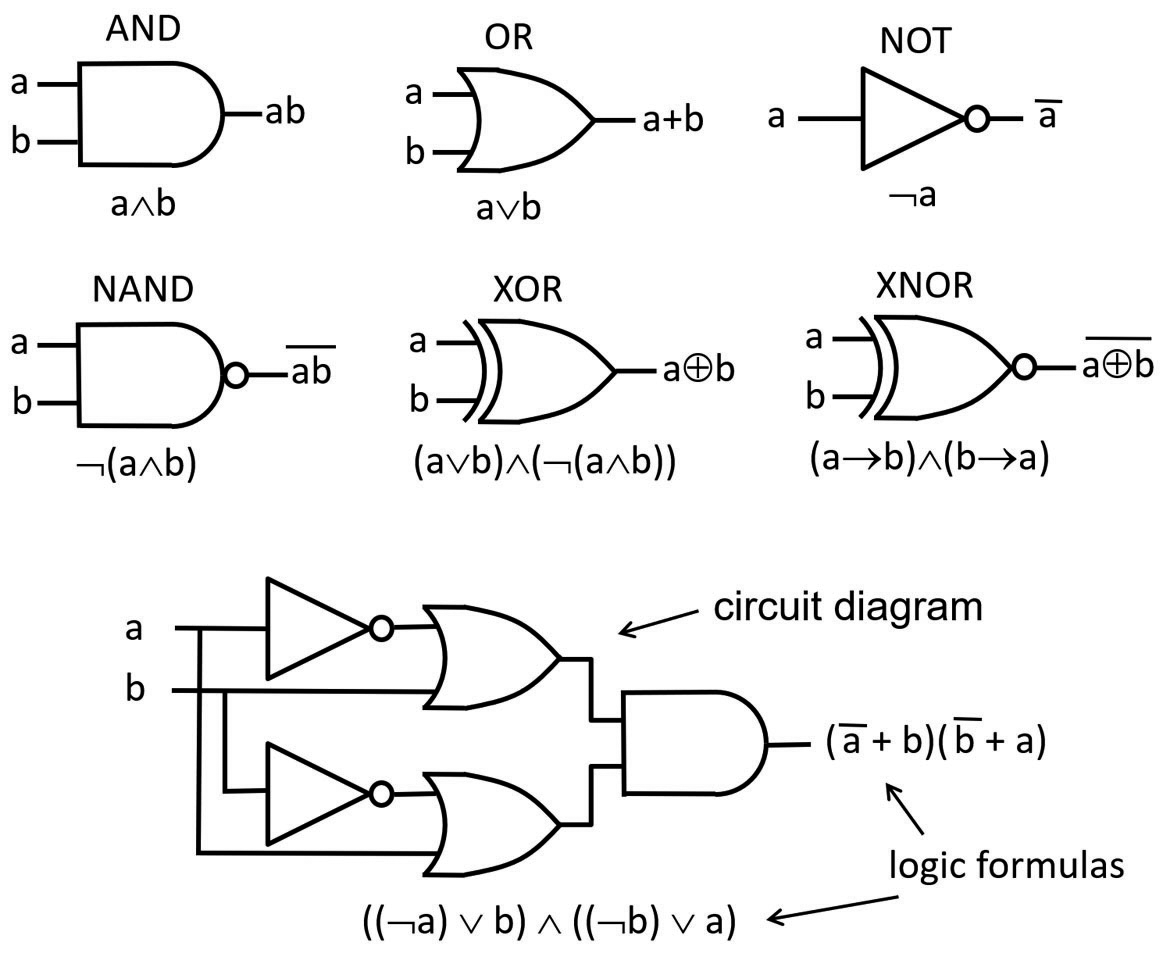
\includegraphics[scale=1]{images-cmyk/LogicGates}
%\todo{I did not have Visio with me. Improvised with PowerPoint. Figure will need to be redrawn.}
\end{center}
\index{gate!logic}\index{Boolean!gate}
\index{circuit!diagram}\index{diagram!circuit}
\index{circuit!Boolean}\index{Boolean!circuit}\index{logic!formula}\index{formula!logic}
\index{negation (not, logic gate)}\index{not (logic gate)}
\index{and (logic gate)}
\index{or (logic gate)}
\index{nand!logic gate}
\index{xor (logic gate)}
\index{xnor (logic gate)}
\index{exclusive or}\index{or, exclusive}
\index{operator, logic!nand}
\index{operator, logic!and ($\wedge$)}
\index{operator, logic!or ($\vee$)}
\index{operator, logic!nor}
\index{operator, logic!not ($\neg$)}
\index{operator, logic!exclusive or}
\index{operator, logic!exclusive nor}
\index{gate!and}
\index{gate!or}
\index{gate!not}
\index{gate!negation}
\index{inverter, gate}
\index{gate!nand}
\index{gate!nor}
\index{gate!xnor}
\index{gate!xor}
\index{gate!inverter}
\caption{Digital Circuits = Logic Formulas}
\label{fig-02-logic-gates}
\end{figure}

Figure~\ref{fig-02-logic-gates} (page \pageref{fig-02-logic-gates})
presents symbols used for logic gates in circuit diagrams
and annotates them with both
the algebraic notation used by circuit designers
and the logic formulas we have been using.
The important fact to remember is that all three notations
\index{circuit!diagram}\index{diagram!circuit}
represent the same concepts in logic. Circuit diagrams, logic formulas,
and the algebraic notation used by circuit designers are three
different notations for exactly the same mathematical objects.
In this sense, digital circuits, and, therefore, computers,
are materializations of logic formulas.
Computers are
\index{logic!in action}logic in action.

The logic operators that we have been using
($\wedge$, $\vee$, $\neg$, $\rightarrow$)
make it possible to write a formula
that delivers precisely the values in the truth table
for any given formula.
The \{implication\} axiom
(Figure~\ref{fig-02-boolean-axioms}, page \pageref{fig-02-boolean-axioms})
expresses implication in terms of logical-or
and negation, which means we lose no expressive power by
discarding implication from the set of logic operations.

Surprisingly, the reverse is also true.
That is, for any given input/output relationship that can be expressed
in a formula using logical-and, logical-or, and negation,
there is an equivalent logic formula using implication as
the only operator. The new formula, using only the
implication operator, produces the same results
as the original formula.
The \{$\neg$ as $\rightarrow$\} equation
(Figure~\ref{some-boolean-theorems}, page \pageref{some-boolean-theorems})
provides a start in this direction by showing how to express
negation in terms of the implication operator.
Furthermore, implication is not the only logic operator
that is universal in this sense.
Another one
is the negation of logical-and, which is called
\index{nand!logic gate}\index{operator, logic!nand}\emph{nand}.
When fabricated using certain widespread technologies,
nand gates can run faster and be more reliable than other gates,
so many integrated circuits make frequent use of nand gates.

It is interesting to see how to put together digital
circuits for basic operators
($\wedge$, $\vee$, and $\neg$) using only nand gates.
Consider negation, for example.
Negation has only one input signal, and nand has two.
Feeding the same signal into both
inputs of a nand gate produces the behavior of
the negation operator,
as the following equation confirms.

\begin{center}
\begin{tabular}{ll}
$(\neg a) = (\neg (a \wedge a))$  & \{$\neg$ as nand\}\label{neg-as-nand}
\end{tabular}
\end{center}

In this way a \index{gate!nand}\index{operator, logic!nand}\index{nand!logic gate}nand gate can serve in place of a
negation gate (also known as an \index{inverter, gate}\index{gate!inverter}\emph{inverter}).
There is a one-step proof of the equation,
citing the \{$\wedge$ idempotent\} theorem
(page \pageref{and-idempotent}).

A nand-only circuit for logical-and can be
\index{logic!gate}\index{gate!logic}\index{universal gate}\index{gate!universal}put
together from two nand gates in sequence.
The signal from the first nand gate is inverted
by feeding it into both inputs of a second nand gate.
Algebraically, this circuit corresponds to the following \{$\wedge$ as nand\} equation.
It takes a two-step proof to verify the equation.
The first step converts the outside nand to negation using the
\{$\neg$ as nand\} equation, and the second step cites
the \{double negation\} axiom from Figure~\ref{fig-02-boolean-axioms}
(page \pageref{fig-02-boolean-axioms}).

\begin{center}
\begin{tabular}{ll}
$(a \wedge b) = (\neg ((\neg (a \wedge b)) \wedge (\neg (a \wedge b))))$ & \{$\wedge$ as nand\}\label{and-as-nand}
\end{tabular}
\end{center}

\index{negation (not, logic gate)}\index{not (logic gate)}Negation took one nand gate and
logical-and took two.
Logical-or can be implemented with three nand gates,
as shown in the following equation,
which can be verified using
the \{$\neg$ as nand\} equation, DeMorgan's laws,
and double negation.

\begin{center}
\begin{tabular}{ll}
$(a \vee b) = (\neg ((\neg(a \wedge a)) \wedge (\neg(b \wedge b))))$ & \{$\vee$ as nand\}\label{or-as-nand}
\end{tabular}
\end{center}

Figure~\ref{fig-02-nand-is-all-you-need} (page \pageref{fig-02-nand-is-all-you-need})
diagrams the digital circuits
corresponding to the formulas that express logical-and, logical-or, and negation
in terms of nand operations.

\begin{figure}
\begin{center}
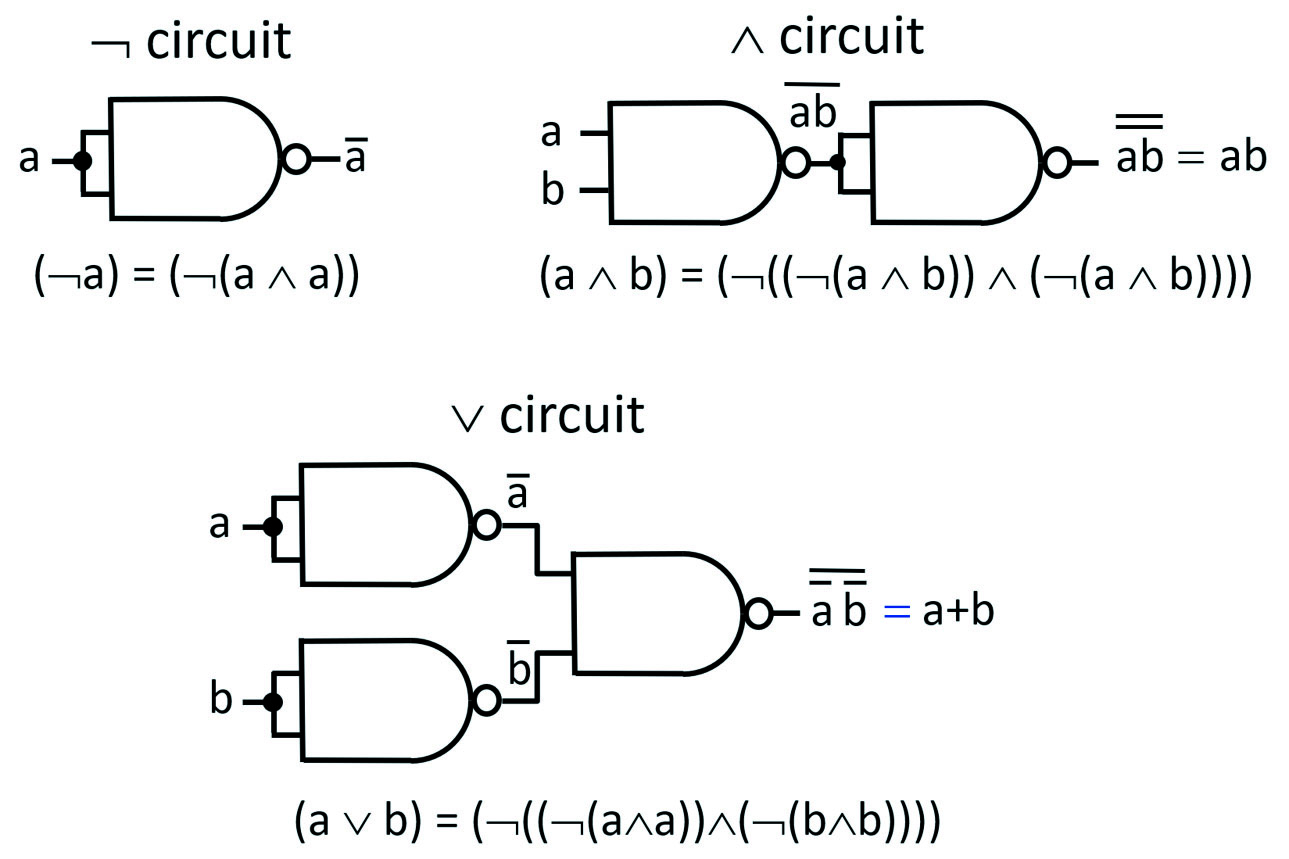
\includegraphics[scale=1]{images-cmyk/NandIsAllYouNeed}
%\todo{I did not have Visio with me. Improvised with PowerPoint. Figure will should be redrawn.}
%% redrew diagram ... still used PowerPoint, but improved the diagram a little 8Aug2017
\end{center}
\index{universal gate}
\index{gate!universal}
\index{nand!logic gate}\index{nand!is all you need}
\index{diagram!circuit}\index{circuit!diagram}
\caption{Nand is All You Need}
\label{fig-02-nand-is-all-you-need}
\end{figure}

\begin{exercises}
\exer {\label{ex:implication-gate}%
Using a negation-gate and an or-gate,
draw a circuit diagram for an ``implication circuit''
that has the same input/output behavior as the implication operator.\\
\emph{Hint}: Follow the example of the \{implication\} axiom
(Figure~\ref{fig-02-boolean-axioms}, page \pageref{fig-02-boolean-axioms})).
One of the inputs will need to be a constant rather than a variable.}

\exer {For each of the following logic formulas,
draw an equivalent circuit diagram.
Since we don't have a symbol for an implication gate,
you can either make up you own symbol or
materialize logic gates where you need them
using the circuit diagram from Exercise \ref{ex:implication-gate}.
\begin{center}
\begin{tabular}{l}
$((a \vee (b \wedge (\neg a))) \vee (\neg (a \vee b)))$ \\
$(((\neg a) \wedge (\neg b)) \wedge (b \wedge (\neg c)))$ \\
$(a \rightarrow (b \rightarrow c))$ \\
$((a \wedge b) \rightarrow c)$ \\
\end{tabular}
\end{center}}

\exer {Rewrite each of the formulas in the previous exercise
in the algebraic notation used by electrical engineers:
juxtaposition for $\wedge$, + for $\vee$, and $\overline{a}$ for $(\neg a)$.
Use the \{implication\} axiom to represent
implications using negation and logical-or.}

\exer {Draw circuit diagrams with behavior
of the and-gate, the or-gate, and the negation-gate
using implication operators only.}
\end{exercises}

%\todo{ do we still want to add half-adder and/or full-adder
%circuits as examples? problem: they have two outputs, so need to talk about
%tapping outputs from subformulas to show correspondence to algebraic form}

\begin{aside}{aside:struggling}{Struggling? Join the Club}
Reasoning with Boolean equations requires a lot of intellectual effort.
Almost everyone struggles when trying to master the concepts
and apply them to solve problems.
So, if you're \index{struggling?}struggling, you're normal.
If you get discouraged to the point of despair, you're normal.
It gets easier with every successful solution, but it never gets easy.
What you are doing here is real mathematics, and it places the same
kind of burden on the intellect as real \index{engineering}engineering.
Engineering is the application of principles
of math and science to the design of useful things,
so real engineering and real mathematics share a great deal of common ground.

If it does not appeal to you to struggle through many
failed attempts and beyond them to a solution, only to
go on to the next problem and start the process once again,
you are going to find engineering to be an unpleasant activity.
It's frustration, frustration, frustration
ad nauseam, then a solution, then on to the next problem.
Finding the solution through all of that fog
brings a lot of satisfaction, and for engineers and mathematicians,
that satisfaction makes it all worthwhile.

So, take heart. Keep trying.
\index{panic, don't}Hundreds of students have worked their way through the reading
and exercises of this chapter and the ones that follow,
and almost all of them have succeeded.
To do so, they invested a great deal of energy in solving problems,
reading, again and again, the examples, and applying the ideas.
Sometimes it takes many hours, just to solve one problem.
Don't give up.\index{panic, don't}\index{disheartened?}\index{frustrated?}\index{baffled?}\index{worried?}\index{scared?}\index{funk, in a?}
%\caption{Struggling? Join the Club}
%\label{aside:struggling}
\end{aside}

\section{Deduction}
\label{sec:deduction}

We have been reasoning with equations,
which means we are reasoning in two directions
at the same time. Equations go both ways.
Deductive \index{reasoning!deductive}\index{deductive reasoning}reasoning is one-directional.
It derives a conclusion from hypotheses using one-directional rules of inference.
A proof shows that the conclusion is true whenever the hypotheses are true, but provides
no information about the conclusion when the truth of one or more of the hypotheses is
unknown.

In the following discussion of proof by \index{deduction!proof by}deduction,
theorems will be stated using the symbol ``$\vdash$'',
which is called a \index{turnstile ($\vdash$)}\emph{turnstile},
to separate the \index{hypothesis!theorem}hypotheses
from the \index{conclusion!theorem}conclusions.
Hypotheses go on the left of the turnstile and the conclusion on the right.
All of the hypotheses are formulas in logic, as is the conclusion.
A turnstile asserts that there is a derivation of the conclusion
from the hypotheses using the rules of inference.
The commutativity law for logical-and, for example,
can be stated as follows.
\begin{center}
\index{theorem, by name!\{$\wedge$ commutes\}}\index{commutative}
Theorem \{$\wedge$ commutes\}: $a \wedge b \vdash b \wedge a$
\end{center}

Later, we will prove the \{$\wedge$ commutes\} theorem using a formal apparatus
for deductive reasoning known as
\index{natural deduction}\index{deduction!natural}\emph{natural deduction}.\footnote{Natural
deduction is a \index{formalism}formal system of logic pioneered in the 1930s
by the mathematician, \index{Gentzen, Gerhard}Gerhard Gentzen, and refined in the 1960s
by the logician, \index{Prawitz, Dag}Dag Prawitz.}
\index{theorem}Theorems proved by natural deduction have zero or more
logic formulas on the left of the turnstile and exactly one formula on the right.
The formulas on the left are the \index{hypothesis}\emph{hypotheses} of the theorem, and
the one on the right is the \index{conclusion}\emph{conclusion}.
A \index{proof}proof begins with the formulas on the left,
which are assumed to be true.
At each step the proof cites either a rule of inference or a previously proven theorem
to derive a new formula. The rule or theorem ensures that when the hypotheses are true,
so is the derived formula. Derived formulas can play the role of hypotheses
in subsequent steps of the proof, and new formulas can be derived from them
in the same manner. The derived formula at the end of the proof is the conclusion.
A deductive proof of a theorem with hypothesis $h$ and conclusion $c$
verifies that the implication $(h \rightarrow c)$ is true.
\begin{center}
$h \vdash c$ ~~ensures that~~ $(h \rightarrow c) = True$
\end{center}

\begin{figure}
\begin{spacing}{0.9}
\begin{center}
\begin{tabular}{ll}
Prove $a$                                               & Prove $a \vee b$                                  \\
 - - - - - -                                            &  - - - - - - - - - -                              \\
Prove $b$                                               & Prove $a \rightarrow c$                           \\
--------------\{$\wedge$ introduction\}                 &  - - - - - - - - - -                              \\
Infer $a \wedge b$                                      & Prove $b \rightarrow c$                           \\
                                                        & -----------------\{$\vee$ elimination\}           \\
                                                        & Infer $c$                                         \\
Prove $a$                                               &                                                   \\
--------------\{$\vee$ introduction 1\}                 &                                                   \\
Infer $a \vee  b$                                       & Prove $a \wedge b$                                \\
                                                        & ----------------\{$\wedge$ elimination 1\}        \\
                                                        & Infer $a$                                         \\
Prove $b$                                               &                                                   \\
--------------\{$\vee$ introduction 2\}                 &                                                   \\
Infer $a \vee  b$                                       & Prove $a \wedge b$                                \\
                                                        & ----------------\{$\wedge$ elimination 2\}        \\
                                                        & Infer $b$                                         \\
Prove $a \rightarrow False$                             &                                                   \\
-----------------------\{$\neg$ introduction\}          &                                                   \\
Infer $\neg a$                                          & Prove $\neg a$                                    \\
                                                        & ---------------------\{$\neg$ elimination\}       \\
                                                        & Infer $a \rightarrow False$                       \\
Prove $a$                                               &                                                   \\
----------\{identity\}                                  &                                                   \\
Infer $a$                                               & Prove \emph{False}                                \\
                                                        & ---------------\{contradiction\}                  \\
                                                        & Infer $a$                                         \\
Prove $a$                                               &                                                   \\
 - - - - - - - - - -                                    &                                                   \\
Prove $a \rightarrow b$                                 & Prove $(\neg a) \rightarrow$ \emph{False}         \\
-----------------\{modus ponens\}                       & --------------------------\{reductio ad absurdum\}\\
Infer $b$                                               & Infer $a$                                         \\
                                                        &                                                   \\
\end{tabular}
\end{center}
\begin{center}
\begin{tabular}{ll}
Assume $a$                                      & \emph{assumption required to cite} \{$\rightarrow$ introduction\}     \\
--------------\{\emph{r}\}                      & \emph{r is an inference rule or proven theorem}                       \\
Prove $b$                                       & $b$ \emph{has now been derived from assumption} $a$                   \\
-----------------\{$\rightarrow$ introduction\} & \emph{proof above line begins with} ``Assume \emph{left operand''}    \\
Infer $a \rightarrow b$                         & ~~~~\emph{and concludes with right operand, proving} $a \rightarrow b$\\
Discharge $a$                                   & \emph{excludes formula} ``$a$'' \emph{from hypotheses of theorem}     \\
\end{tabular}
\end{center}
\end{spacing}
\index{hypothesis!Assume (natural deduction)}
\index{Assume (natural deduction)}\index{proof!Assume (natural deduction)}
\index{inference rule, by name!\{$\wedge$ introduction\}}
\index{inference rule, by name!\{$\vee$ introduction 1\}}
\index{inference rule, by name!\{$\vee$ introduction 2\}}
\index{inference rule, by name!\{$\vee$ elimination\}}
\index{inference rule, by name!\{$\neg$ introduction\}}
\index{inference rule, by name!\{identity\}}
\index{inference rule, by name!\{modus ponens\}}
\index{inference rule, by name!\{$\wedge$ elimination 1\}}
\index{inference rule, by name!\{$\wedge$ elimination 2\}}
\index{inference rule, by name!\{$\neg$ elimination\}}
\index{inference rule, by name!\{contradiction\}}
\index{inference rule, by name!\{reductio ad absurdum\}}
\index{inference rule, by name!\{$\rightarrow$ introduction\}}
\index{inference rule!table of}
\index{modus ponens}
\index{contradiction!inference rule}
\seeonlyindex{elimination rule}{inference rule}
\seeonlyindex{introduction rule}{inference rule}
\index{identity}
\index{reductio ad absurdum}
\index{deductive proof}
\index{natural deduction}
\index{deduction!natural}
\index{discharge assumption}\index{Assume (natural deduction)!discharge}\index{hypothesis!discharge}
\index{inference rule!discharge assumption}
\index{proof!deductive}
\caption{Rules of Inference for Natural Deduction}
\label{fig-02-deduction-rules}
\end{figure}

Of course the truth of an implication formula doesn't
say anything about the value of the
left-hand operand of the implication operator.
That value could be either $True$ or $False$.
The implication formula just says that
the only combination of values that can make
$(h \rightarrow c)$ have the value $False$
(namely, $h = True$, $c = False$, as verified in
Theorem \{$\rightarrow$ truth table\},
page \pageref{implication-truth-table}) cannot occur.
In the same way, a deductive proof of a theorem
does not provide any information about the hypotheses.
It only says that the conclusion will be true
whenever all of the hypotheses are true.

\begin{figure}
%\begin{quote}
Theorem \{Socrates was mortal\}: $man$, $man \rightarrow mortal$ $\vdash$ $mortal$ \\
\emph{proof}
%\end{quote}
\begin{center}
\begin{spacing}{0.9}
\begin{tabular}{l}
Assume $man$                    \\
 - - - - - - - - - - - - - - - - - -\\
Assume $man \rightarrow mortal$ \\
--------------------------------\{modus ponens\} \\
~~~~~~ $mortal$                 \\
\end{tabular}
\end{spacing}
\end{center}\index{inference rule, by name!\{modus ponens\}}\index{modus ponens}\index{Socrates syllogism}\index{syllogism!Socrates}\index{theorem!Socrates}\index{Assume (natural deduction)}
\caption{Theorem \{Socrates Was Mortal\}: Citing Modus Ponens}
\label{fig:socrates-proof}
\end{figure}

Sometimes a theorem has several hypotheses.
A proof by deductive reasoning of the theorem
$h_1$, $h_2$ $\vdash$ $c$,
which has two hypotheses,
ensures that
$((h_1 \wedge h_2) \rightarrow c) = True$.
A theorem with no hypotheses at all
would have no formulas on the left-hand side of the turnstile:
$\vdash c$.
A proof of such a theorem would
verify the equation $c = True$.

All of the axioms of Boolean algebra
(Figure~\ref{fig-02-boolean-axioms}, page \pageref{fig-02-boolean-axioms})
can be derived through deductive reasoning.
Many presentations of classical logic begin with
\index{deductive reasoning}deductive \index{reasoning!deductive}reasoning,
but we started with Boolean algebra
because we will be using logic to reason about
digital circuits and software specified in the form of equations.
So, equations play a central role throughout the
discussion.\footnote{An accessible,
more extensive discussion of natural deduction can be found
in O'Donnell, Hall, and Page,
\emph{Discrete Mathematics Using a Computer}
(2\textsuperscript{nd} ed.), Springer, 2006.}

Figure~\ref{fig-02-deduction-rules} (page \pageref{fig-02-deduction-rules})
provides schematics of the rules of inference of \emph{natural deduction}.
A citation of an inference rule derives a \index{conclusion}new formula
from hypotheses (assumed true) or formulas derived through prior reasoning in the proof.
Each \index{citation!inference rule}\index{inference rule!citation}rule citation
has three parts:
%\begin{quote}
\begin{enumerate}
\item a proof above the line (or multiple proofs, depending on the rule),
\item a line annotated with the name of the cited inference rule, and
\item exactly one logic formula below the line.
\end{enumerate}
%\end{quote}

\label{def-deductive-proof}
A \emph{deductive proof} is a sequence of citations of inference rules
in which the final citation has, below the line,
the formula that is the conclusion of the theorem that the proof verifies.
An inference rule can place specific constraints on the formula
that is its conclusion and/or on the formulas that are the
conclusions of the proofs that the rule requires above the line.
For example, the \{$\wedge$ elimination 1\} inference rule
(Figure~\ref{fig-02-deduction-rules}, page \pageref{fig-02-deduction-rules})
requires one \index{proof!deductive}proof
\index{proof!above/below the line}above the line
and constrains the conclusion of that proof
to be a logical-and formula $(a \wedge b)$.
The \{$\wedge$ introduction\} rule, on the other hand,
requires two proofs above the line and
constrains its conclusion (below the line)
to be a logical-and formula $(a \wedge b)$.
Some rules place constraints both on the formulas
above the line (which have been derived earlier in the proof)
and on the formula
\seeonlyindex{above the line}{proof}\seeonlyindex{below the line}{proof}\index{line (natural deduction)!above/below}below the line.
For example the \{$\neg$ introduction\} rule requires
the formula above the line to be an implication
whose conclusion is the logical constant \emph{False}
($a \rightarrow False$)
and constrains the formula below the line to be
a negation formula ($\neg a$).
Furthermore, the hypothesis of the implication above the line must be the same
formula that is negated below the line.

When a rule is
\index{citation!inference rule}\index{inference rule!citation}\seeonlyindex{rule of inference}{inference rule}cited
in a deductive proof,
the name of the rule is written just to the right of
the line that separates the proofs that the rule requires above the line
from the conclusion that the citation derives,
which is the formula written below the line.
When an inference rule requires multiple proofs above the line,
dashed lines separate those proofs.
Each of the proofs that the rule requires above the line
is, itself, a proof.
That is, it is also a sequence of citations ending in a conclusion formula.

The \index{scope!inference rule citation}\index{inference rule!scope of citation}\emph{scope} of a
\index{citation!inference rule}\index{inference rule!citation}citation
of an inference rule
extends upward to the beginning of the first of the proofs
above the line that the rule requires.
The scopes of citations in a proof can overlap,
and when they do, some proofs are nested inside others.
In fact, the scope of the last rule citation in a proof
always extends upward to the beginning of the proof,
so the scopes of all of the other citations are nested
within the scope of the last citation.\footnote{Because
of nested scopes,
proofs by natural deduction
are sometimes written with parentheses,
like algebraic formulas,
or displayed as ``tree diagrams'',
with the conclusion of the theorem at the bottom and
the citations spread out, upwards,
in a branching structure
that makes the overlapping (and non-overlapping)
of scopes easy to see.
We have chosen a vertical format with implicit
overlapping because this notation is more compact than a
\index{natural deduction!tree diagram}\index{proof!tree diagram}tree
diagram and, in our judgment,
more readable than a parenthesized proof formula.}

Wherever an inference rule requires a proof above the line,
an assumption can take the place of that proof.
That is,
an assumption can always stand in lieu of a proof.
A logic formula that is marked as an assumption
is a hypothesis of the theorem verified by the proof
(unless that assumption is subsequently \emph{discharged},
a special dispensation
that will be discussed later).
So, any proof may begin with a formula
that is marked as an assumption.
However, no proof can have
a formula marked as an assumption after
the first rule citation in the proof.
\index{proof!assumption}Assumptions
can appear only above the line
of the first citation in the sequence of citations
comprising the proof, but since citations
(and, therefore, proofs) can be nested,
an assumption need not be the first line in
the entire proof.
It may, instead, be the first line
in a proof that is nested inside another proof.

The \index{modus ponens}\{modus ponens\} rule
(Figure \ref{fig-02-deduction-rules}, page \pageref{fig-02-deduction-rules})
is probably the most widely recognized rule of inference because
of the well known ``Socrates was mortal'' syllogism
(Figure \ref{fig:socrates-proof}, page \pageref{fig:socrates-proof}).
The rule says that if there is a proof concluding in
the formula $a$ and a proof concluding in the formula ($a \rightarrow b$),
those proofs, together with a citation of modus ponens,
derive the conclusion $b$.\footnote{Deductive
proofs are one-directional,
and so is the theorem about Socrates.
One can conclude mortality from two hypotheses about circumstances of life,
but one cannot derive those circumstances from the mortality of Socrates.
Rabbits, for example, are mortal, but they are not men.}

Proofs by natural deduction follow strictly a prescribed format,
and it is worth going over that format again, in slightly different terms.
The proof of a theorem that has
$n$ hypotheses will have $n$ different
formulas representing those hypotheses
marked as assumptions
at the beginning of one or more of the proofs
required by the inference rules that the proof cites.
That is, each hypothesis, at the point where it is introduced
into the proof, is marked as an assumption.
An assumption, so marked, stands in lieu of the proof
required at that point by whatever inference rule is being cited.
A particular formula in a proof may be marked as an assumption
at more than one point in a proof, but no matter how many places
it appears as an assumption, it is still just
one hypothesis of the theorem being proved.
A proof of a theorem with $n$ hypotheses will have at least $n$
formulas marked as assumptions.
It will have more than $n$ formulas marked as assumptions
if two or more of the assumptions specify the same formula
(or if a formula is discharged).

Assumptions must appear at the beginning of a
a proof, before the citation of any
inference rule in the proof.
Assumptions cannot pop up after the citation
of an inference rule in a proof.
Of course, since \index{proof!dashed line}\index{line (natural deduction)!dashed}dashed
lines indicate separate proofs,
the \index{Assume (natural deduction)}assumption need not be at the beginning of the entire
proof, but could, instead, be at the beginning of
a proof separated from another proof by a dashed line.
The \{Socrates was mortal\} theorem
(Figure \ref{fig:socrates-proof})
has two hypotheses.
One is marked as an assumption standing in lieu of the first proof
required by a citation of \{modus ponens\},
and the other is marked as an assumption
standing in lieu of the second proof
required by \{modus ponens\}.

Three of the inference rules of natural deduction
(Figure \ref{fig-02-deduction-rules})
involve the $\wedge$ operator:
\{$\wedge$ introduction\},
\{$\wedge$ elimination 1\}, and
\{$\wedge$ elimination 2\}.
Using these rules, we can construct a deductive proof
of the commutativity law for $\wedge$,
and the proof will serve as a reasonably straightforward
example to get started with natural deduction.

\begin{figure}
Theorem \{$\wedge$ commutes\}: $a \wedge b$ $\vdash$ $b \wedge a$ \\
\emph{proof}
\begin{center}
\begin{spacing}{0.9}
\begin{tabular}{ll}
Assume $a \wedge b$                             &\emph{hypothesis of theorem}\\
-------------------\{$\wedge$ elimination 2\}   &\\
~~~~~~~~~~$b$                                   &\emph{concludes 1$^{\text{st}}$ proof for} \{$\wedge$ introduction\}\\
 - - - - - - - - - - - - - - - - - - - - - - - -&\emph{separates proofs for} \{$\wedge$ introduction\}\\
Assume $a \wedge b$                             &\emph{hypothesis of theorem (reused)}\\
-------------------\{$\wedge$ elimination 1\}   &\\
~~~~~~~~~~$a$                                   &\emph{concludes 2$^{\text{nd}}$ proof for} \{$\wedge$ introduction\}\\
-------------------\{$\wedge$ introduction\}    &\emph{scope extends to top}\\
~~~~~~~~$b \wedge a$                            &\emph{proved} $b$, \emph{proved} $a$, \emph{conclude} $(b \wedge a)$\\
\end{tabular}
\end{spacing}
\end{center}\index{hypothesis!Assume (natural deduction)}\index{Assume (natural deduction)}\index{proof!Assume (natural deduction)}\index{inference rule, by name!\{$\wedge$ elimination 2\}}\index{inference rule, by name!\{$\wedge$ elimination 1\}}\index{inference rule, by name!\{$\wedge$ introduction\}}\index{proof!deductive}\index{theorem, by name!\{$\wedge$ commutes\}}\index{commutative}
\caption{\{$\wedge$ commutes\}: Citing Three Inference Rules Involving $\wedge$}
\label{fig:and-commutes-proof}
\end{figure}

The proof in
Figure \ref{fig:and-commutes-proof} (page \pageref{fig:and-commutes-proof})
cites the \{$\wedge$ introduction\} inference rule,
a rule that requires two proofs above the line.
The first of those proofs, in this example, has the hypothesis
of the theorem above the line, marked as an assumption.
It then cites the \{$\wedge$ elimination 2\} rule,
which requires the right-hand operand ($b$) of the $\wedge$
above the line to go under the line as the conclusion.
Then comes the dashed line separating
the two proofs required by \{$\wedge$ introduction\}.
The second of the proofs comes next.
It has the same form as the first proof,
except that it cites \{$\wedge$ elimination 1\} instead of \{$\wedge$ elimination 2\}.
The \{$\wedge$ elimination 1\} rule brings the left-hand operand ($a$) of the $\wedge$
down below the line.
The \{$\wedge$ introduction\} rule requires the
conclusion of the first proof above line to
become the left-hand operand of the $\wedge$
operation that the rule introduces,
and it requires the conclusion of the second
proof to be the right-hand operand.
The $\wedge$ formula with those two operands
is the conclusion below the line citing the \{$\wedge$ introduction\} inference rule.
That final citation completes the proof of the \{$\wedge$ commutes\} theorem.

To recap, the proof of the {\{$\wedge$ commutes\} theorem
consisted of three proofs, in a sense,
one being the whole proof, ending in the citation of
the \{$\wedge$ introduction\} rule,
and the other two being the proofs required by the citation of \{$\wedge$ introduction\}.
Each of the three proofs in this example consisted of exactly one rule citation.
Sometimes there are several rule citations in a proof, sometimes only one,
and, when the proof is an assumption, none.

\begin{aside}{variable-stand-for-formulas}{Variables Stand for Formulas}
As in Boolean algebra, variables in deductive reasoning
stand for arbitrary formulas.
Any grammatically correct formula
can be plugged in for a variable in a theorem,
as long as all of the instances of that variable are
replaced by that same formula.
For example,
Theorem \{$\wedge$ commutes\} ($a \wedge b$ $\vdash$ $b \wedge a$)
has two variables, $a$ and $b$.
Since ($x \vee y$) and ($y \rightarrow z$) are formulas,
the theorem justifies the following, more specialized
version.
\begin{center}
$(x \vee y) \wedge (y \rightarrow z)$ $\vdash$ $(y \rightarrow z) \wedge (x \vee y)$
\end{center}
The theorem also justifies the following restatement of the
theorem that uses the formula $b$ in place of $a$ and the formula $a$ in place of $b$.
\begin{center}
$b \wedge a$ $\vdash$ $a \wedge b$
\end{center}
Variables are used in this manner throughout the book. Nothing new here.
We bring it up again because it is important
to keep in mind when citing inference rules
or theorems.\index{variable}\index{formula!variables}
%\caption{Variables Stand for Formulas}
%\label{variable-stand-for-formulas}
\end{aside}

Two formulas are annotated as assumptions in the
proof of the \{$\wedge$ commutes\} theorem.
This suggests that the theorem has
two hypotheses,
but in this case both assumptions are the same formula.
A particular formula can be used as many times as necessary as
an assumption in a proof, but it only counts as one hypothesis
in the theorem.
The number of hypotheses
of the theorem is the number of distinct
formulas annotated as assumptions in the proof,
minus the number of those assumptions that are discharged
by citations of the \{$\rightarrow$ introduction\} inference rule,
which we will discuss shortly.

\begin{figure}
Theorem \{self-implication\}: $\vdash$ $a \rightarrow a$ ~~~~\emph{Note: This theorem has no hypotheses.}\\
proof
\begin{center}
\begin{spacing}{0.9}
\begin{tabular}{ll}
Assume $a$                  &\emph{assumption discharged later}\\
---------------\{identity\} &\\
~~~~~$a$                    &\\
---------------\{$\rightarrow$ introduction\} &\\
~~$a \rightarrow a$         &\emph{assumed} $a$\emph{, proved} $a$\emph{, conclude} $a \rightarrow a$\\
~~Discharge $a$             &\emph{discharged by} \{$\rightarrow$ introduction\} \emph{citation}, \emph{as promised}\\
\end{tabular}
\end{spacing}
\end{center}\index{hypothesis!Assume (natural deduction)}\index{Assume (natural deduction)}\index{proof!Assume (natural deduction)}\index{inference rule, by name!\{identity\}}\index{inference rule, by name!\{$\rightarrow$ introduction\}}\index{hypothesis!discharge}\index{discharge assumption}\index{Assume (natural deduction)!discharge}\index{inference rule!discharge assumption}\index{theorem, by name!\{self-implication\}}
\caption{$\vdash$ $a \rightarrow a$: Citing  \{identity\} and \{$\rightarrow$\ introduction\} Inference Rules}
\label{fig:or-self-imp-proof}
\end{figure}

Given a proof, it is straightforward to extract
the theorem it proves.
On the left of the turnstile ($\vdash$) put all of the different
formulas annotated as assumptions in the proof,
except those that are discharged.
After the turnstile, write the formula in the
conclusion at the end of the proof.

Now we come to the issue of
\index{hypothesis!discharge}\index{discharge assumption}\index{Assume (natural deduction)!discharge}\index{inference rule!discharge assumption}\index{proof!discharge assumption}\index{Assume (natural deduction)!discharge}discharging
formulas assumed in proofs.
The inference rule \{$\rightarrow$ introduction\}
has some unique characteristics.
It requires only one proof above the line,
but that proof must begin with a formula
(let's call it $a$)
marked as an assumption.
To repeat, the proof above the line in a citation of
\{$\rightarrow$ introduction\} that
concludes with the formula $(a \rightarrow b)$
below the line
must begin with ``Assume $a$'' and
then continue from there to derive the formula $b$, just above the line.
The scope of the \{$\rightarrow$ introduction\} citation
extends upward to the required assumption.

Normally, any formula assumed at the beginning of a proof
becomes a \index{hypothesis}hypothesis of the theorem that was proved.
However, a
\index{hypothesis!discharge}\index{discharge assumption}\index{Assume (natural deduction)!discharge}\index{inference rule!discharge assumption}\index{proof!discharge assumption}discharged
assumption
is not added to the hypotheses of the theorem.
A citation of the
\index{inference rule, by name!\{$\rightarrow$ introduction\}}\{$\rightarrow$ introduction\} rule
triggers a discharge of the assumed formula that the
rule requires at the beginning of the proof above the line.
(Without that assumption, the citation,
and therefore the proof, is not valid.)
The reason for the discharge is that the truth of an implication
formula doesn't place any constraints on the value of its
left-hand operand.
The implication says that if the left-hand operand
has the value \emph{True}, then so does the right-hand operand,
and the proof confirms that relationship.
Since the citation of the
\{$\rightarrow$ introduction\} rule
simply confirms that the implication formula below the line
is true, the citation places no constraints on the value
of the left-hand operand.
The assumption only applies within the scope
of the citation of the \{$\rightarrow$ introduction\} inference rule
and, therefore, does not become a hypothesis of the theorem being proved
(unless it is assumed elsewhere in the proof and not discharged).

Figure \ref{fig:or-self-imp-proof} (page \pageref{fig:or-self-imp-proof})
displays a proof of the \{self-implication\} theorem,
which says that formulas of the form ($a \rightarrow a$) always have the value \emph{True}.
The proof cites the \{identity\} rule,
which is included among the inference rules to make it
possible for proofs by natural deduction to stay strictly
within the formalism required by the system.
The \{identity\} rule says that a proof of a formula $a$
can be followed by a citation of the \{identity\} rule
with that same formula, $a$, as its conclusion below the line.

The application of any rule must \index{matching!inference rule}\index{inference rule!matching}match
the template in the specification of the rule,
and the \{identity\} rule is sometimes needed to make it possible to match a template.
That is what happens in the proof of self-implication (Figure \ref{fig:or-self-imp-proof}).
The proof cites the \{$\rightarrow$ introduction\} rule
to derive the formula $(a \rightarrow a)$,
and that citation requires
a proof above the line that begins with the assumption of $a$
and concludes with the formula $a$, just above the line.
The \{identity\} rule makes it possible to satisfy this requirement.
In the proof of self-implication,
the citation of
\index{implication ($\rightarrow$)!introduction}\{$\rightarrow$ introduction\} rule
follows the derivation of $a$ from $a$ and triggers a
\index{discharge assumption}discharge
of the assumption of $a$ at the beginning of the proof.
There are no other \index{Assume (natural deduction)}assumed formulas in the proof,
so the theorem proved has no hypotheses.
That is, the \index{proof}proof confirms that the
\index{conclusion}conclusion formula
$(a \rightarrow a)$ has the value $True$, regardless of
what formula $a$ stands for.

\begin{figure}
Theorem \{$\vee$ commutes\}: $a \vee b$ $\vdash$ $b \vee a$ \\
\emph{proof}
\begin{center}
\begin{spacing}{0.9}
\begin{tabular}{ll}
Assume ($a \vee b$)          &\emph{hypothesis of theorem}\\
 - - - - - - - - - - - - - - - - - - - - - -&\emph{separates 1\textsuperscript{st} and 2\textsuperscript{nd} proofs for} \{$\vee$ elimination\} \\
Assume $a$          &\emph{this assumption will be discharged}\\
--------------\{$\vee$ introduction 2\} &\emph{allows arbitrary left-hand operand in conclusion}\\
~~$(b \vee a)$        &\\
-----------------\{$\rightarrow$ introduction\} &\emph{assumed} $a$\emph{, proved} $(b \vee a)$\emph{, conclude} $a \rightarrow (b \vee a)$ \\
~$a \rightarrow (b \vee a)$ &\{$\vee$ elimination\} \emph{requires this conclusion here}\\
Discharge $a$              &\emph{discharged by} \{$\rightarrow$ introduction\} \emph{citation, as promised}\\
 - - - - - - - - - - - - - - - - - - - - - -&\emph{separates 2\textsuperscript{nd} and 3\textsuperscript{rd} proofs for} \{$\vee$ elimination\}\\
Assume $b$          &\emph{this assumption will be discharged}\\
--------------\{$\vee$ introduction 1\} &\emph{allows arbitrary right-hand operand in conclusion}\\
~~$(b \vee a)$        &\\
-----------------\{$\rightarrow$ introduction\} &\emph{assumed} $b$\emph{, proved} $(b \vee a)$\emph{, conclude} $b \rightarrow (b \vee a)$\\
~$b \rightarrow (b \vee a)$ &\{$\vee$ elimination\} \emph{requires this conclusion here}\\
Discharge $b$               &\emph{discharged by} \{$\rightarrow$ introduction\} \emph{citation, as promised}\\
---------------\{$\vee$ elimination\}       &\emph{scope extends up to} Assume $(a \vee b)$\\
~~~~$(b \vee a)$        &\emph{3 req'd proofs above, conclude} $(b \vee a)$\\
\end{tabular}
\end{spacing}
\end{center}
\index{hypothesis!Assume (natural deduction)}\index{Assume (natural deduction)}\index{proof!Assume (natural deduction)}\index{inference rule, by name!\{$\vee$ elimination\}}\index{inference rule, by name!\{$\vee$ introduction 2\}}\index{inference rule, by name!\{$\rightarrow$ introduction\}}\index{inference rule, by name!\{$\vee$ introduction 1\}}\index{inference rule!discharge assumption}\index{discharge assumption}\index{Assume (natural deduction)!discharge}\index{hypothesis!discharge}\index{theorem, by name!\{$\vee$ commutes\}}\index{commutative}
\caption{\{$\vee$ commutes\}: Citing \{$\vee$ elimination\}}
\label{fig:or-commutes-proof}
\end{figure}

We now take on a theorem whose proof is more complex
than those we have studied so far.
The \{$\wedge$ commutes\} theorem proved earlier
is similar to the \{$\vee$ commutes\} theorem
that we will discuss now, but the proofs are very different.
Figure \ref{fig:or-commutes-proof} (page \pageref{fig:or-commutes-proof}),
which displays the proof of the \{$\vee$ commutes\} theorem,
cites all three of inference rules involving the $\vee$ operator
and affords an example of how the \{$\vee$ elimination\} rule works.

The \{$\vee$ elimination\} rule calls for three proofs above the line.
\index{inference rule, by name!\{$\vee$ elimination\}}The
first of the three proofs must conclude in a formula
that is a logical-or, $(a \vee b)$, where, of course,
$a$ and $b$ can be any grammatically correct logic formulas.
The second proof must conclude in an implication, $a \rightarrow c$.
In this implication, $a$ is the left-hand operand of the $\vee$ formula
that concluded the first proof above the line,
and $c$ (which of course can be a formula rather than just a variable)
is the conclusion under the line citing the \{$\vee$ elimination\} rule.
The third proof must conclude in an implication, $b \rightarrow c$,
with the same right-hand operand as the implication that concludes
the second proof, but with a left-hand operand that is the same
as the right-hand operand of the logical-or that concludes the
first proof above the line.
The \{$\vee$ elimination\} rule is complicated,
but is surprisingly easy to cite
because the rule places so many constraints on its various parts.

The proof in Figure~\ref{fig:or-commutes-proof} cites both of the
``or introduction'' rules:
\{$\vee$ introduction 1\} and \{$\vee$ introduction 2\}.
These rules allow the introduction of an arbitrary formula
into the proof.
That is, when you cite the rule, you can make up one of the
formulas in the conclusion (namely, the right-hand operand of
the logical-or in the case of \{$\vee$ introduction 1\}
and the left-hand operand in the case of \{$\vee$ introduction 2\}).
The formula you choose can be as complicated or as simple as you like,
whatever is needed to make the proof work.
In the proof at hand,
the made-up formulas are simple ($b$ in one case and $a$ in the other case),
but are exactly what the proof needs.

In addition to citing all three inference rules involving the $\vee$ operator,
the proof cites the \{$\rightarrow$ introduction\} rule twice.
Both of those citations require discharges,
so there's lot of action in the proof.
Figure~\ref{fig:or-commutes-proof}
elucidates the details with commentary
intended to help you work through the proof
to understand how the citations fit together and
comprise a proof of the \{$\vee$ commutes\} theorem.

Deductive proofs are one-directional,
so it's a little ironic that most
of the theorems we've prove so far using natural deduction
turn out to be bidirectional.
The proofs went in only one direction,
but the theorems were provable in the other direction, too.

The theorem that we turn to now, the implication chain rule
(Figure \ref{fig:impchain-proof}, page \pageref{fig:impchain-proof}),
only goes in one direction.
It derives a conclusion from two hypotheses,
but the two hypotheses cannot be derived from the conclusion.
Again, commentary with the proof is intended
to help you work your way through it.
Pay particular attention to the discharge of the
assumption that is introduced at the top of the proof.

\begin{figure}
Theorem \{$\rightarrow$ chain\}
$(a \rightarrow b)$, $(b \rightarrow c)$ $\vdash$ $a \rightarrow c$ \\
\emph{proof}
\begin{center}
\begin{spacing}{0.9}
\begin{tabular}{ll}
Assume $a$                                             &\emph{assumption discharged later}\\
 - - - - - - - - - - - - - - - - - - - - - - - -       &\emph{separates proofs required by} \{modus ponens\}\\
Assume $a \rightarrow b$                               &\emph{hypothesis of theorem}\\
-----------------------\{modus ponens\}                &\{modus ponens\} \emph{citation} $\dots$\\
~~~~~~~~~~~~$b$                                        &~~~~~\emph{scope of citation extends up to} Assume $a$\\
 - - - - - - - - - - - - - - - - - - - - - - - -       &\emph{separates proofs for second} \{modus ponens\} \\
Assume $b \rightarrow c$                               &\emph{hypothesis of theorem}\\
------------------------\{modus ponens\}               &\emph{second citation of} \{modus ponens\} $\dots$\\
~~~~~~~~~~~~$c$                                        &~~~~~\emph{scope overlaps first citation} \\
------------------------\{$\rightarrow$ introduction\} &\\
~~~~~($a \rightarrow c$)                               &\emph{assumed} $a$\emph{, proved} $c$\emph{, conclude} $(a \rightarrow c)$ \\
~~~~~Discharge $a$                                     &\emph{discharged by citation of} \{$\rightarrow$ introduction\}\\
\end{tabular}
\end{spacing}
\end{center}
\index{hypothesis!Assume (natural deduction)}
\index{Assume (natural deduction)}\index{proof!Assume (natural deduction)}
\index{inference rule, by name!\{modus ponens\}}
\index{inference rule, by name!\{$\rightarrow$ introduction\}}
\index{modus ponens}
\index{theorem, by name!\{$\rightarrow$ chain\}}
\index{inference rule!discharge assumption}
\index{discharge assumption}\index{Assume (natural deduction)!discharge}
\index{hypothesis!discharge}
\caption{Proving the Implication Chain Rule}
\label{fig:impchain-proof}
\end{figure}

In \index{proof!deductive}deductive proofs, previously proven theorems
can be cited as if they were
\index{inference rule!theorem as}\index{theorem!as inference rule}inference rules.
Of course, the proof could always be carried out using inference rules alone
by copying the proof of the cited theorem in place of its citation,
but that leads to very long proofs, just as writing a computer program
without defining and invoking procedures encapsulating common operations
leads to very long programs. Long proofs, like long programs, tend
to be unreliable, maybe because it's so difficult
to analyze such a large mass of
detail without getting confused.
But, even if they weren't unreliable, they would be an eyesore,
not to mention difficult to fix if there were an error.
That's why the ability to cite proven theorems in
deductive proofs is important. It makes them shorter
and easier to comprehend incrementally, one short proof at a time.

\begin{figure}
Theorem \{modus tollens\}: $a \rightarrow b$, $\neg b$ $\vdash$ $\neg a$\\
\emph{proof}
\begin{center}
\begin{spacing}{0.9}
\begin{tabular}{ll}
Assume $a \rightarrow b$                      &\emph{hypothesis of theorem}\\
 - - - - - - - - - - - - - - - - - - - -      &\emph{separates proofs of hypotheses of} \{$\rightarrow$ chain\} \emph{theorem}\\
Assume $\neg b$                               &\emph{hypothesis of theorem}\\
---------------\{$\neg$ elimination\}         &\\
$b \rightarrow False$                         &\\
---------------\{$\rightarrow$ chain\}        & \emph{citing theorem with 2 hypotheses} $\dots$\\
$a \rightarrow False$                         &~~~~~~~~\emph{scope extends to top of proof}\\
---------------\{$\neg$ introduction\}        &\\
~~~~$\neg a$                                  &\\
\end{tabular}
\end{spacing}
\end{center}
\index{hypothesis!Assume (natural deduction)}
\index{Assume (natural deduction)}\index{proof!Assume (natural deduction)}
\index{inference rule, by name!\{$\neg$ elimination\}}
\index{inference rule, by name!\{$\neg$ introduction\}}
\index{modus tollens}
\index{theorem, by name!\{modus tollens\}}
\caption{Modus Tollens: Citing a Theorem to Justify an Inference}
\label{fig:modtol-proof}
\end{figure}

A citation of a theorem in a proof must be preceded by proofs of
each of its hypotheses above the line, just as
each inference rule citation must be preceded by a certain number of proofs above the line.
As with inference rules that require multiple proofs above the line,
we use a dashed line to separate the required proofs
when citing a theorem that has more than one hypothesis and therefore
requires more than one proof above the line.
Figure \ref{fig:modtol-proof} (page \pageref{fig:modtol-proof})
displays a proof of the modus tollens theorem.\footnote{The
inference rule \{modus ponens\} says that the conclusion of an implication
can be derived from a proof of its hypothesis.
The modus tollens theorem says that the hypothesis
of an implication can be derived from
a proof of the negation of its conclusion.}
The proof cites the implication chain rule theorem.
Since that theorem has two hypotheses, there are two proofs above
the line where the theorem is cited. Those proofs conclude in
the implication formulas that are the hypotheses of the implication chain rule.
Finally, the a citation of the \{$\neg$ introduction\} rule completes the proof.

The \{reductio ad absurdum\} rule supports
``proof by contradiction.''
It says that if you can prove that the formula
$(\neg a) \rightarrow$ \emph{False} is true
you can conclude that the formula $a$ is true.
The proof in Figure~\ref{fig:dbl-neg-fwd} (page \pageref{fig:dbl-neg-fwd})
cites the
\index{proof!reductio ad absurdum}\index{inference rule, by name!\{reductio ad absurdum\}}\index{reductio ad absurdum}reductio
ad absurdum rule to prove a theorem about double negation.

\begin{figure}
Theorem \{$\neg \neg$ forward\}: $(\neg(\neg a))$ $\vdash$ $a$\\
\emph{proof}
\begin{center}
\begin{spacing}{0.9}
\begin{tabular}{ll}
Assume $(\neg(\neg a))$                       &\emph{hypothesis of theorem}\\
----------------------\{$\neg$ elimination\}  &\\
~~$(\neg a) \rightarrow False$                &\\
----------------------\{reductio ad absurdum\}&\emph{proved} $(\neg a) \rightarrow False$, \emph{conclude} $a$\\
~~~~~~~~~~~~$a$                               &\\
\end{tabular}
\end{spacing}
\end{center}
\index{hypothesis!Assume (natural deduction)}
\index{Assume (natural deduction)}\index{proof!Assume (natural deduction)}
\index{inference rule, by name!\{$\neg$ elimination\}}
\index{inference rule, by name!\{reductio ad absurdum\}}
\index{proof!by contradiction}
\index{contradiction!proof by}
\index{theorem, by name!\{$\neg \neg$ forward\}}
\caption{\{$\neg \neg$ forward\}: Citing Reductio ad Absurdum}
\label{fig:dbl-neg-fwd}
\end{figure}

Citations in the example proofs, so far, have included all of the inference rules
but one. The rule we haven't used yet is \{contradition\}.\footnote{It
is ironic that proofs citing the \{reductio ad absurdum\} rule
are called proofs by contradiction, while proofs citing the
\{contradiction\} rule have no special name.
Nevertheless, that is the custom, maybe because
the \{contradiction\} rule, like the \{identity\} rule,
is needed primarily to facilitate the formalities of
natural deduction.}
The proof of the \{disjunctive syllogism\} theorem displayed in
Figure~{\ref{fig:disjunctive-syllogism-nd} (page \pageref{fig:disjunctive-syllogism-nd})
exhibits a citation of that rule.
The theorem says that if a logical-or is known to be true,
and its left-hand operand is known to be false,
then its right-hand operand must be true.
The strategy of the proof employs the \{$\vee$ elimination\} rule,
which calls for three proofs above the line.
The first of those proofs is simply an assumption of
the logical-or formula that is a hypothesis of the theorem.
The second proof derives $False$ from the other hypothesis
of the theorem and an assumption of the left-hand operand
of the logical-or. That assumption is discharged when
the proof cites the \{$\rightarrow$ introduction\} rule.
The third proof is similar to the second proof,
but cites the \{identity\} rule at the point
corresponding to the citation of the \{contradition\} rule in second proof.

Creating proofs by
\index{proof!deductive}\index{natural deduction}natural deduction is hard.
It requires a lot of practice, just to get
a firm grasp of the ideas.
The following exercises provide an opportunity
to get some of that practice. As a
\index{natural deduction!where to start}\index{rule of thumb!natural deduction}\index{deduction!rule of thumb}rule of thumb,
it often helps to start at the bottom
of a proof by natural deduction. Write the conclusion formula
at the bottom (it will have to go there, anyway),
and draw a line above it. Choose an inference rule that
might be cited on that line, and think about how you might
be able to cite the rule, possibly considering the hypotheses of
the theorem you are trying to prove or other formulas
that might be derivable from them. Working from the bottom
of the proof in this way can be an effective strategy for
finding the insights needed to create a proof.

\begin{figure}
Theorem \{disjunctive syllogism\}: $a \vee b$, $\neg a$ $\vdash$ $b$ \\
\emph{proof}
\begin{center}
\begin{spacing}{0.9}
\begin{tabular}{ll}
Assume $(a \vee b)$          &\emph{hypothesis of theorem}\\
 - - - - - - - - - - - - - - - - - - - - - -&\emph{separates 1\textsuperscript{st} and 2\textsuperscript{nd} proofs for} \{$\vee$ elimination\}\\
Assume $a$          & \emph{this assumption will be discharged}\\
 - - - - - - - - - - - - - - - - - - - - - -& \emph{separates 1\textsuperscript{st} and 2\textsuperscript{nd} proofs for} \{modus ponens\} \\
Assume $(\neg a)$        & \emph{hypothesis of theorem}\\
-------------------\{$\neg$ elimination\} \\
~~$a \rightarrow False$ &\\
-----------------\{modus ponens\} &\emph{scope extends up to} Assume $a$\\
~~~~$False$            &\{contradiction\} \emph{rule requires} $False$ \emph{just above the line}\\
-----------------\{contradiction\} &\emph{citing this rule justifies any conclusion}\\
~~~~~~~~$b$              &\emph{now we have derived $b$ from} Assume $a$\\
-----------------\{$\rightarrow$ introduction\} & \emph{assumed $a$, proved $b$, conclude $(a \rightarrow b)$}\\
~~~~$a \rightarrow b$ &\emph{conclusion required by citation of} \{$\vee$ elimination\} \\
Discharge $a$    &\emph{discharged by citing} \{$\rightarrow$ introduction\}\emph{, as promised}\\
 - - - - - - - - - - - - - - - - - - - - - -&\emph{separates 2\textsuperscript{nd} and 3\textsuperscript{rd} proofs for} \{$\vee$ elimination\}\\
Assume $b$          &\emph{this assumption will be discharged}\\
--------------\{identity\} &\\
~~~~~~~~$b$          &\\
-----------------\{$\rightarrow$ introduction\} &\emph{assumed $b$, proved $b$, conclude $(b \rightarrow b)$}\\
~~~~$b \rightarrow b$ &\emph{conclusion required by citation of} \{$\vee$ elimination\}\\
Discharge $b$              & \emph{discharged by citing} \{$\rightarrow$ introduction\}\emph{, as promised}\\
---------------\{$\vee$ elimination\}       &\emph{requires three proofs the above, scope goes to top}\\
~~~~~~~~$b$        &\emph{proved} $(a \vee b)$\emph{,} $(a \rightarrow b)$\emph{, and} $(b \rightarrow b)$\emph{, conclude} $b$\\
\end{tabular}
\end{spacing}
\end{center}
\index{hypothesis!Assume (natural deduction)}
\index{Assume (natural deduction)}\index{proof!Assume (natural deduction)}
\index{inference rule, by name!\{$\vee$ elimination\}}
\index{inference rule, by name!\{modus ponens\}}
\index{inference rule, by name!\{$\neg$ elimination\}}
\index{inference rule, by name!\{contradiction\}}
\index{inference rule, by name!\{$\rightarrow$ introduction\}}
\index{inference rule, by name!\{identity\}}
\index{inference rule!discharge assumption}
\index{discharge assumption}\index{Assume (natural deduction)!discharge}
\index{hypothesis!discharge}
\index{theorem, by name!\{disjunctive syllogism\}}
\index{disjunctive syllogism}
\index{syllogism!disjunctive}
\caption{\{disjunctive syllogism\}: Citing \{contradiction\}}
\label{fig:disjunctive-syllogism-nd}
\end{figure}

\begin{exercises}

\exer {\label{thm:and-complement}%
Use natural deduction to prove
\index{theorem, by name!\{$\wedge$ complement\}}Theorem
\{$\wedge$ complement\}: $a$, $\neg a$ $\vdash$ $False$}

\exer {\label{ex:dbl-mod-pon}%
Use natural deduction to prove the following theorem:
$a$, $a \rightarrow b$, $b \rightarrow c$ $\vdash$ $c$}

\exer {\label{ex:dbl-mod-pon-eq}%
Derive the equation
$((a \wedge ((a \rightarrow b) \wedge (b \rightarrow c))) \rightarrow c)$ = $True$
using the axioms of Boolean algebra
(Figure~\ref{fig-02-boolean-axioms}, page \pageref{fig-02-boolean-axioms}).}

\exer {Explain the connection between
Exercises~\ref{ex:dbl-mod-pon} and \ref{ex:dbl-mod-pon-eq}.}

\exer {
Use natural deduction to prove the following theorem:
$\vdash$ $(a \wedge b) \rightarrow a$}

\exer {\label{ex:nor-commutes}%
Use natural deduction to prove
\index{theorem, by name!\{nor commutes\}}\index{nor!commutes}\index{commutative}Theorem
\{nor commutes\}: $\neg (a \vee b)$ $\vdash$ $\neg (b \vee a)$\\
\emph{Note}: The \{$\vee$ commutes\} theorem will not help because
$\neg (a \vee b)$ is a negation formula, not a logical-or formula.
It has a logical-or as a subformula, but natural deduction
requires matching the whole formula, not a subformula.}

\exer {Use natural deduction to prove
\index{theorem, by name!\{nand commutes\}}\index{nand!commutes}\index{commutative}Theorem
 \{nand commutes\}: $\neg (a \wedge b)$ $\vdash$ $\neg (b \wedge a)$\\
\emph{Note}: The \{$\wedge$ commutes\} theorem will not help in this proof
for the same reason that \{$\vee$ commutes\} does not help
in Exercise~\ref{ex:nor-commutes}.}

\exer {Use natural deduction to prove
\index{theorem, by name!\{nor elimination 1\}}\index{nor!elimination}Theorem
\{nor elimination 1\}: $\neg (a \vee b)$ $\vdash$ $\neg a$}

\exer {\label{ex:DeMfwd}%
Use natural deduction to prove
\index{DeMorgan}\index{theorem!DeMorgan}\index{theorem, by name!\{DeMorgan $\vee$ forward\}}\{DeMorgan $\vee$ forward\}:
$\neg (a \vee b)$ $\vdash$ $(\neg a) \wedge (\neg b)$}

\exer {\label{ex:DeMbkw}%
Use natural deduction to prove
\index{DeMorgan}\index{theorem!DeMorgan}\index{theorem, by name!\{DeMorgan $\vee$ backward\}}\{DeMorgan $\vee$ backward\}:
$(\neg a) \wedge (\neg b)$ $\vdash$ $\neg (a \vee b)$}

\exer {Explain the connection between Exercises~\ref{ex:DeMfwd} and \ref{ex:DeMbkw}.\\
\emph{Hint}: Review Box~\ref{aside:boolean-equivlance} (page \pageref{aside:boolean-equivlance}).}


\exer {Use natural deduction to prove\index{theorem, by name!\{$\vee$ complement\}}
Theorem \{$\vee$ complement\}: $\vdash$ $a \vee (\neg a)$ \\
\emph{Hint}: Use the \{reductio ad absurdum\} inference rule,
cite the \{nor elimination 1\} and \{$\wedge$ complement\}
theorems from earlier exercises,
and remember that you can assume the hypothesis
of the theorem as many times in the proof as you like.}

\exer {The proof of the \{disjunctive syllogism\} theorem in Figure~\ref{fig:disjunctive-syllogism-nd}
(page \pageref{fig:disjunctive-syllogism-nd})
would be shorter if it cited the \{self-implication\} theorem
(Figure~\ref{fig:or-self-imp-proof}, page \pageref{fig:or-self-imp-proof})
to derive the formula $(b \rightarrow b)$ instead of using the
\{identity\} and \{$\rightarrow$ introduction\} inference rules
to derive that formula.
Change the proof to make it shorter in this way.}

\end{exercises}

%index tags to this point, 2nd pass, 26Nov2017

\section{Predicates and Quantifiers}
\label{sec:predicates-and-quantifiers}

\label{proposition-def}
We have been using the term \index{proposition}\emph{proposition}
to mean a formula that is either true or false.
Any set\footnote{The
term
\index{set}``set'' has a checkered history in mathematics.
It is tricky to define in a way that avoids contradictions
like Russell's paradox, which you can read about
in online articles or textbooks.
Instead of dwelling on those issues,
we are going to assume that,
for any of the sets that we talk about,
we have a way of figuring out whether any given
item is an element of the set or not.
Usually, our sets will be familiar ones,
such as the set of natural numbers, which
is the universe of discourse indexing the propositions
in proofs by mathematical induction, or
the set of lists that can be constructed
by an ACL2 program.
Occasionally, the universe of discourse will be
the set of all programs that can be expressed in a given
programming language.
In that case
any interpreter for the language
can determine whether or
not a given item is in the set.}
of propositions is called,
when the set is taken as a whole, a
\label{predicate-def}\index{predicate}\emph{predicate}.
We will require a predicate
to be a collection of propositions
indexed by a set known as the
\label{def-universe-of-discourse}\index{universe of discourse}\emph{universe of discourse}.
If $P$ is a \index{predicate!universe of discourse}predicate, and $x$ is an element from
the universe of discourse, then $P(x)$ is
the \index{proposition}\index{proposition!vs predicate}\index{predicate!vs proposition}proposition
selected from the predicate by the index $x$.\footnote{You
can think of the predicate as an
operator that delivers the associated proposition as output
when supplied with the index of the proposition as input,
such as the ACL2 operator natp: (natp $x$) is true if
$x$ is a natural number and false otherwise.
No matter whether you look at it as a set of propositions
indexed by a universe of discourse or an operator that
delivers a true/false value given an element of the universe of discourse,
the predicate is the same mathematical entity.
The indexed-set approach is sometimes called an \index{extensional}``extensional'' view
because it focuses on the externally observable characteristics of the predicate,
while the operator perspective is called an \index{intensional}``intensional'' view
because it involves the internal workings of a way to produce the true/false value
of a proposition, given its index.
Occasionally, a predicate will not correspond to a computation,
and in that case the operator (intensional) view
isn't valid because there will be no
computation associated with the predicate.
The extensional view is the way
to think about predicates of that kind.}

If we write a formula that connects some of the propositions
of the predicate \emph{P} with logical-and
$(P(x_1) \wedge P(x_2) \wedge P(x_3) \wedge P(x_4))$,
the formula has the value $True$
when all of the propositions in the formula ($P(x_1)$, $P(x_2)$, $P(x_3)$, $P(x_4)$)
are $True$.
We would like to be able to write a formula
for the logical-and of all the propositions in the predicate \emph{P}.
We could do this with an ordinary logical-and formula,
but this gets bulky when there are a lot of elements
in the universe of discourse,
and it's impossible when the universe of discourse
has an infinite number of elements.

The usual way to write the logical-and of all the propositions in a predicate
makes use of a symbol that looks like an upside-down letter A
and is known as the
\label{def:universal-quantifier}\index{universal quantifier ($\forall$)}\index{quantifier!$\forall$, forall}\index{quantifier!universal ($\forall$)}\index{forall ($\forall$)}\emph{universal quantifier} ($\forall$).
The  formula $(\forall x.P(x))$
stands for the logical-and of all the propositions in the predicate
\emph{P}.\footnote{The
formula $(\forall x. P(x))$ reads ``for all $x$, $P(x)$ is \emph{True}.''}
The value of the formula is $False$
if there is an element $x$ from the universe of discourse
for which the proposition $P(x)$ is $False$.
Otherwise, $(\forall x.P(x))$ is $True$.

For example, suppose $n$ stands for a natural number
and we take use
$E(n)$ as a shorthand for the proposition ``$2n$ is a non-negative, even number''.
Then \{$E(0)$, $E(1)$,$E(2)$, \dots\}
is a set of propositions indexed by the natural numbers.
For each natural number $n$, there is a corresponding proposition $E(n)$,
so \emph{E} is a predicate with the natural numbers
as its universe of discourse.

If we write a formula that connects some of these propositions with $\wedge$
$(E(5) \wedge E(3) \wedge E(7) \wedge E(1))$,
the formula has the value $True$
because all four of those propositions are $True$.
In fact all of the propositions in the predicate E are $True$.
$E(n)$ is $True$, regardless of which natural number $n$ stands for,
because any number of the form $2n$ is a non-negative, even number
when $n$ is a natural number.
Therefore, there is no element $n$ in the universe of discourse of
the predicate $E$ for which the proposition $E(n)$ is $False$,
which means that the value of the quantified formula $\forall n.E(n)$
is $True$.

A
\label{def:quantifier}
\index{quantifier}quantifier converts a set of propositions (that is, a predicate)
into a single value, true or false. That is, a quantifier converts
a predicate to a proposition.
Syntactically, a quantified formula starts with a quantifier symbol followed by
a variable, then a period, and finally a logic formula
representing a proposition. The variable,
which is known as the
\label{def:bound-variable}
\index{bound variable}\index{variable!bound}\emph{bound variable}
in the formula, stands for an
element of the universe of discourse, and the quantification
ranges over the entire universe of discourse.
The universe of discourse is not specified directly
in the formula, but the formula has no meaning unless
the universe of discourse is known.

\begin{aside}{empty-forall}{Quantifier with Empty Universe}
Let $P$ be a predicate.
The formula
$\forall x.P(x)$
is false when there is
at least one index $x$ in the universe of discourse
for which $P(x)$ is false.
Otherwise, the $\forall$ quantification is true.
If the universe of discourse is empty,
there aren't any indexes at all,
let alone one for which the predicate is false.
Therefore, $\forall x.P(x)$ is true
when the universe of discourse is empty.

Using a similar rationale, a
$\exists$ quantification
is false when the universe of discourse is empty
because it can only be true if there is
at least one element, $x$, in the universe of discourse
for which $P(x)$ is true.\index{universal quantifier ($\forall$)!empty universe}\index{forall ($\forall$)!empty universe}\index{existential quantifier ($\exists$)!empty universe}\index{there exists ($\exists$)!empty universe}\index{quantifier!empty universe}
%\caption{Quantifier with Empty Universe}
%\label{empty-forall}
\end{aside}

Any variable that is not bound is
called a
\index{bound variable}\index{variable!free}\index{variable!bound}\index{free variable}\label{def:free-variable}\emph{free variable}.
In the formula $(\forall x.P(x)) \vee y$,
$x$ is a bound variable, and $y$ is a free variable.
This can get a bit tricky, but you have to keep it
straight to understand how quantifiers work.
An especially tricky case is the formula
$(\forall x.P(x)) \vee x$.
In this formula, $x$ is a bound variable in the
operand on the left-hand side of the $\vee$,
but is a free variable on the right-hand side.

The only other quantifier we will use is the
\label{def:existential-quantifier}\index{existential quantifier ($\exists$)}\index{quantifier!$\exists$, there exists}\index{quantifier!existential ($\exists$)}\index{there exists ($\exists$)}\emph{existential quantifier}.
It forms the logical-or of all the propositions in a predicate
and is represented by a symbol that looks like a backwards letter E.
The  formula $(\exists x.P(x))$
has the value $True$
if there is an element $x$ from the universe of discourse
for which the proposition $P(x)$ is $True$.\footnote{The
formula $(\exists x.P(x))$ reads
``there exists $x$ such that $P(x)$ is \emph{True}.''}

Consider the equation $((n + 7) = 12)$.
Any equation is a proposition because it is either
$True$ or $False$. Let's call this proposition $Q(n)$.
We can take the view that $Q$ is a predicate
with the natural numbers as its universe of discourse
because for each natural number $n$,
$Q(n)$ stands for a proposition.
You know from algebra that there is a natural number
$n$ for which equation $((n + 7) = 12)$ holds.
That is, there is a value (namely, the number $n=5$) in the universe
of discourse for which the proposition $Q(n)$ is $True$.
Therefore, according to the definition of the
existential quantifier,
the formula $(\exists n.Q(n))$ is $True$.

The formula $(\forall n.Q(n))$, however, is $False$
because there is a natural number $n$ for which
the proposition $Q(n)$ is $False$.
In fact there are many of them, but
the number of $False$ propositions in the predicate doesn't matter
in a universal quantification. One is enough.
By the definition of the universal quantifier,
the formula $(\forall n.Q(n))$
is $False$ if there is even one element of the
universe of discourse for which the proposition
$Q(n)$ is $False$.

\begin{aside}{aside:ch02-three-line-equal}{Equal by Definition: $\equiv$}
The three-line variation of the equals sign
indicates that the term on the left stands
for the formula on the right, \emph{by definition}.
\begin{center}
\index{equation!defining ($\equiv$)}\index{definition!equation ($\equiv$)}\index{equal, three-line ($\equiv$)}\index{equivalence!by definition ($\equiv$)}\index{three-line equal ($\equiv$)}
\begin{tabular}{ll}
$term \equiv \dots \emph{some formula} \dots$ & ~~~~~ \emph{definition of term} \\
$Q(n) \equiv ((n + 7) = 12)$                  & ~~~~~ $Q(n)$ \emph{stands for} $((n + 7) = 12)$ \\
\end{tabular}
\end{center}
%\caption{Equal by Definition: $\equiv$}
%\label{aside:ch02-three-line-equal}
\end{aside}

Predicates can have more than one index.
For example, the \index{predicate}\index{predicate!multi-index}predicate $R$,
defined as follows, has two indexes.
\begin{center}
$R(m, n) \equiv ((n + 7) = m)$
\end{center}
In this discussion the universe of discourse
for both indexes will be the natural numbers.\footnote{A
predicate with multiple indexes can
have different universes of discourse for different indexes.
One index could come from a set of numbers
and the other from a set of words, for example,
but both the first and second indexes
of the particular predicate $R$ discussed here
are natural numbers.}
For each pair of natural numbers $(n, m)$,
$R(n, m)$ stands for a proposition (namely the
equation $((n + 7) = m)$, which is either $True$ or $False$).
The formula $(\exists n.R(n,m))$ is a different
proposition for each natural number $m$.
That makes it a set of propositions indexed by the natural numbers,
so it is a predicate with the natural numbers as its universe of discourse.
To keep things straight, let's give this predicate a name.
\begin{center}
$S(m) \equiv (\exists n.R(n,m))$
\end{center}

Let's convert this predicate to a proposition by quantifying it:
$(\forall m.S(m))$. This is a proposition, so
it is either $True$ or $False$, but which is it?
By the definition of the predicate $R$,
$S(m)$ would be $True$ if there were no natural numbers $m$
for which the quantification $(\exists n.((n+7) = m))$ were $False$.
Suppose $m$ is the natural number zero.
The proposition $S(0)$ says $(\exists n.((n+7) = 0))$.
There are no natural numbers $n$ such that
$((n+7) = 0))$ because $n$ would have to be negative,
and all natural numbers are zero or bigger.
Therefore, $S(0)$ is $False$,
and that makes $(\forall m.S(m)) = False$.

By definition
$S(m)$ stands for the formula $(\exists n.R(n,m))$,
so we can put that formula in place of $S(m)$
in $(\forall m.S(m))$. When we do this,
the formula becomes $(\forall m.(\exists n.R(n,m)))$,
in which an existential quantification
is nested inside a universal quantification.
It can go the other way, too, and with any
combination of quantifiers.
All of the following formulas are propositions,
and with your understanding of numbers, you
can figure out which ones are $True$ and
which are $False$.
\begin{center}
$(\exists m.(\forall n.R(n,m)))$ \\
$(\exists m.(\exists n.R(n,m)))$ \\
$(\forall m.(\forall n.R(n,m)))$
\end{center}
Nested quantifications like this are common
when a predicate has multiple indexes.

\begin{exercises}
\exer {Work out the values of the following formulas,
where $R(m, n) \equiv ((n + 7) = m)$.
\subexer {$(\exists m.(\forall n.R(n,m)))$}
\subexer {$(\exists m.(\exists n.R(n,m)))$}
\subexer {$(\forall m.(\forall n.R(n,m)))$}

}

\exer {Mark the
\index{free variable}\index{bound variable}\index{variable!free}\index{variable!bound}free
variables in the following formulas and say how many bound variables
each formula has.
\subexer {$(x \vee (y \rightarrow z))$}
\subexer {$(\forall x.(P(x) \wedge (\forall y.Q(y))))$}
\subexer {$(x \rightarrow (\exists y.Q(y)))$}
\subexer {$(\exists x.(P(x) \wedge (\forall y.Q(y))))$}
\subexer {$((\forall x.(P(x) \rightarrow Q(y))) \vee (\forall x.W(x)))$}
\subexer {$(\forall x. (\forall z.R(x, y, z)))$}
}

\end{exercises}

\section{Reasoning with Quantified Predicates}
\label{sec:quantifier-equations}

Quantifiers provide a way to convert predicates to propositions,
and you have some experience in reasoning about Boolean formulas constructed with
propositions and operators.
This section discusses some new methods and equations to make
the same kind of reasoning possible with formulas containing quantifiers.

Let's start with a predicate $P$ with two indexes.
$P(x,y)$ will denote the proposition in the predicate $P$ that is indexed
by the pair $(x,y)$, where $x$ comes from the universe of discourse for the first index
and $y$ from the universe of discourse for the second index.

In our discussion, we will want to provide some examples
of specific values in the universe of discourse.
We could do this by making up some special symbols for those values,
but to keep things uncomplicated at this point,
let's say that natural numbers are the universe of discourse for both indexes.
That will give us familiar symbols for particular indexes.
$P(5,2)$, $P(0,6)$, and $P(3,7)$ would be specific propositions in the predicate $P$.
$P(x,y)$ would also be a proposition in predicate $P$, but would not be a specific one
unless we knew which natural numbers $x$ and $y$ stood for.
Again, we chose natural numbers as the universe of discourse
only to make it easy to designate specific elements in the domain.
The points we make in the discussion about reasoning with quantified predicates
would be the same for other choices of the universe of discourse.

Suppose we have already proved that the formula $(\forall x.(P(5, x)))$ is $True$.
How can we use this predicate in another proof?
One way is to observe that $(\forall x.(P(5, x)))$ means that all of the formulas
$P(5, 0)$, $P(5, 1)$, $P(5, 2)$, \dots are $True$,
so we can assert in a proof that, for example,
$P(5, 0) = True$. We could also assert that $P(5, 1)$ is $True$, and $P(5, 2)$, and so on.
That is, once we have proved that a universally quantified formula has the value $True$,
we can use that to justify a more specific theorem that
eliminates the quantifier and replaces the bound variable by any specific value
in the universe of discourse.

Not only that, but we could replace the variable by any formula
representing a value in the universe of discourse.
For example, we could assert that if $x$ and $y$ denote natural numbers,
then $(\forall x.(P(5, 2x + y + 4)))$ is $True$.

Another formula to consider is the existential quantification $(\exists x.(P(5, x)))$.
Suppose we know it has the value $True$, and we want to make use of that fact in a proof.
The meaning of the formula $(\exists x.(P(5, x)))$ is that
there is at least one $x$ from the universe of discourse that makes the expression $True$,
but it doesn't say which one.
It could be that $P(5, 9)$ is $True$, or that $P(5, 3)$ is $True$,
or any other proposition in $P$ whose index is a pair with $5$ as its first component.
It could be exactly one of them,
or just two or three, or it could even be all of them, but
there must be at least one. That's all we know
from a proof that $(\exists x.(P(5, x)))$ is $True$.

One way to make use of that fact is to use a notational convention
to indicate that what looks like a variable (which could stand for any
value in the universe of discourse or even a formula representing such a value)
is not really a variable, but is, instead, a specific value in the universe of
discourse. That is, the symbol is a constant, not a variable.
One way to do this would be to designate a special symbol, capital $C$ perhaps,
to use when we want to indicate that what looks like a variable is really a constant.
\label{def:skolem-constant}
If we need several different constants in our discussion, we could use different
subscripts: $C_x$, $C_y$, $C_{197}$, $C_{\xi}$, etc.
Another approach is to use subscripts on ordinary variables ($x_0$, $y_8$, \dots)
to indicate that the symbols stand for constants, not variables.
The important thing is (1)~to say in the commentary of the proof that the new
symbol stands for a specific value from the universe of discourse and is not a variable
and (2)~to make sure to use a new symbol for each new constant and to not use that
symbol for any other purpose in the proof.
In any case, what was a bound variable
%(page \pageref{def:bound-variable})
in an existential quantification
becomes a free constant in the formula that represents a particular proposition in the
predicate, and it is a proposition that has the value $True$.

So what about proofs? How can we prove a statement that uses quantifiers?
One approach is to systematically
remove the quantifiers, so as to produce a formula that has no quantifiers.
In other words, we
are left with formula without variables, such as $P(5,3)$ or $P(5,x_0)$ where
$x_0$ stands for a particular element in the universe of discourse whose value
we don't know, but which in any case stands for just one value and cannot
be replaced by another variable or formula.
Since there are no variables, this is really just a Boolean formula
for an ordinary proposition,
so it can be proved using the same methods we used
with Boolean propositions.

This approach to reasoning about quantified formulas is a four-step process
(Figure~\ref{fig:four-step-quantifier-reasoning}, page \pageref{fig:four-step-quantifier-reasoning}).
The last step is the already familiar area of reasoning
with Boolean formulas that represent propositions,
but the first three steps involve new ideas.

\begin{figure}
\begin{center}
\begin{tabular} {ll}
~&Step 1. Rename bound variables \\
~&Step 2. Migrate quantifiers \\
~&Step 3. Eliminate quantifiers (leaving a proposition) \\
~&Step 4. Prove theorem about the proposition \\
\end{tabular}
\label{four-step-strategy-quantifiers}
\index{Skolemization}
\index{quantifier!reasoning with}
\index{reasoning!with quantifiers}
\end{center}
\caption{A Four-Step Strategy for Reasoning with Quantifiers}
\label{fig:four-step-quantifier-reasoning}
\end{figure}

Renaming bound variables, which is the first step, is sometimes necessary to prevent
a quantifier from accidentally referring to a different bound variable
that happens to have the same name.
For example, consider the formula
$(\forall x.Odd(x)) \vee (\forall x.Even(x))$,
where the universe of discourse for both quantifiers is the integers.\footnote{$Odd(x) \equiv (\exists y.(x = 2y+1))$.
\label{even-number-predicate-Even}
$Even(x) \equiv (\exists y.(x = 2y))$.
These formulas define the predicates $Odd$ and $Even$.
The integers are the universe of discourse,
both for the predicates (variable $x$)
and for the quantifications (bound variable $y$).}
This formula has the value $False$ because there
is an integer $x$ for which $Odd(x$) is false (the number $2$, for example).
That makes $(\forall x.Odd(x))$ false.
Similarly, $(\forall x.Even(x))$ is false,
and since both operands of $\vee$ in $(\forall x.Odd(x)) \vee (\forall x.Even(x))$
are false, the formula is false (\{$\vee$ truth table\},
Figure~\ref{or-truth-table}, pagee \pageref{or-truth-table}).
There are two bound variables in the formula.
These are different variables even though they both have
the same name, $x$.
The formula $(\forall x.(Odd(x) \vee Even(x)))$, on the other hand,
has only one bound variable and is true.
We have to be careful to keep these formulas straight.
They look similar, but they have totally different meanings.

Another important aspect of quantified formulas is that
the name of a bound variable has no affect on the value
of the formula:
$(\forall x.Even(x))$ has the same meaning
as $(\forall y.Even(y))$.
So, to avoid conflating two different bound variables,
we start by choosing names for the bound variables
so that each quantification uses a bound variable of a different name.
For example, in the formula
$(\forall x.Odd(x)) \vee (\forall x.Even(x))$,
we could change the name of the bound variable
in the second quantification:
$(\forall x.Odd(x)) \vee (\forall y.Even(y))$.
The meaning of the formula remains the same,
but the change of name prevents confusion between two different bound variables.

Suppose we have a quantified formula that contain
many variables: $(\forall x.(P(\dots x \dots)))$.
How do we rename the bound variable $x$ in this formula?
First, we insist on using a completely new name,
one that does not appear else in the formula.
This is for the same reason as before: we do not want to confuse the variable
$x$ with a different variable that happens to have the same name.
Choosing a new name for $x$ that is the same as the name
of some other variable would defeat our purpose.

Second, we must ensure that when we
change the name of the bound variable $x$ to, say,
$y$, we replace all occurrences of that bound variable $x$ with $y$.
However, we must be careful not to change
any occurrence of a different variable
that happens also to have the name $x$.
For example, recall that there are two different, but identically named,
bound variables in the formula
$(\forall x.Odd(x)) \vee (\forall x.Even(x))$.
We would want to change one of them to a new name, such as $y$.
That would produce either the formula
$(\forall x.Odd(x)) \vee (\forall y.Even(y))$ or the formula
$(\forall y.Odd(y)) \vee (\forall x.Even(x))$.

For example, suppose we are trying to prove that
if $P$ is a predicate with two indexes,
%% rlp 12/7/17: I DON'T THINK THE HYPOTHESIS ABOUT SAME UNIV OF DISCOURSE IS NEEDED
%%that have the same universe of discourse,
then the following formula has the value $True$.
$$((\exists y. (\forall x. P(x, y))) \rightarrow (\forall x. (\exists y. P(x, y)))) = True$$

The formula has four different bound variables
but only two different names.
We need to rename two of them to avoid conflicts.
That the first step in our four-step strategy.
We apply the equation \{R$\exists$\} from
Figure~\ref{fig-02-quantifiers} (page \pageref{fig-02-quantifiers})
to justify renaming the bound variable $y$ in $\exists y$
in the left-hand operand of the implication.
Any name is okay, as long as it is not already present in the formula.
We choose $v$ and get a new formula
that, according to equation \{R$\exists$\}, has the same value as
the formula we started with.
%\begin{center}
%\begin{tabular}{ll}
%$((\exists y. (\forall x. P(x, y))) \rightarrow (\forall x. (\exists y. P(x, y)))) =
% ((\exists v. (\forall x. P(x, v))) \rightarrow (\forall x. (\exists y. P(x, y))))$ & \{R$\exists$\} \\
%\end{tabular}
%\end{center}
$$((\exists y. (\forall x. P(x, y))) \rightarrow (\forall x. (\exists y. P(x, y)))) =
 ((\exists v. (\forall x. P(x, v))) \rightarrow (\forall x. (\exists y. P(x, y)))) ~~ \{R\exists\}$$

Next, we rename the bound variable \emph{x} in $\forall x$
on the left of the implication.
We change $x$ to $u$, again choosing a name that differs
from all the other variable names in the formula.
\begin{center}
\begin{tabular}{ll}
$((\exists v. (\forall x. P(x, v))) \rightarrow (\forall x. (\exists y. P(x, y)))) =
  (\exists v. (\forall u. P(u, v))) \rightarrow (\forall x. (\exists y. P(x, y)))$ & \{R$\forall$\} \\
\end{tabular}
\end{center}

We now have four variables in the formula: $u$, $v$, $x$, and $y$.
Each quantifier is associated with a bound variable of a different name,
so we won't mix up the roles of the variables.
The next step is to migrate the quantifiers to the front of the formula.
Then the implication will be inside the scope of all the quantifiers:
$(\forall x.(\forall v.(\exists u.(\exists y.(\dots\rightarrow\dots)))))$.
The equations in Figure~\ref{fig-02-quantifiers}
provide the basis for quantifier migration.
Applying the equations in a proof calls for a close look
at parentheses to be sure that the cited equation from
the figure matches the syntax of the formula that is under scrutiny.
Migrating quantifiers is a tedious process and requires
careful attention to detail.

\begin{figure}
\begin{center}
\begin{tabular}{ll}
$((\forall x.P(\dots x \dots)) \wedge Q) = (\forall x.(P(\dots x \dots) \wedge Q))$               & \{$\forall\wedge$\} \\
$((\exists x.P(\dots x \dots)) \wedge Q) = (\exists x.(P(\dots x \dots) \wedge Q))$               & \{$\exists\wedge$\} \\
$((\forall x.P(\dots x \dots)) \vee Q) = (\forall x.(P(\dots x \dots) \vee Q))$                   & \{$\forall\vee$\} \\
$((\exists x.P(\dots x \dots)) \vee Q) = (\exists x.(P(\dots x \dots) \vee Q))$                   & \{$\exists\vee$\} \\
$((\forall x.P(\dots x \dots)) \rightarrow Q) = (\exists x.(P(\dots x \dots) \rightarrow Q))$     & \{${\forall}{\rightarrow}$\} \\
$((\exists x.P(\dots x \dots)) \rightarrow Q) = (\forall x.(P(\dots x \dots) \rightarrow Q))$     & \{${\exists}{\rightarrow}$\} \\
$(Q \rightarrow (\forall x.P(\dots x \dots))) = (\forall x.(Q \rightarrow P(\dots x \dots)))$     & \{${\rightarrow}{\forall}$\} \\
$(Q \rightarrow (\exists x.P(\dots x \dots))) = (\exists x.(Q \rightarrow P(\dots x \dots)))$     & \{${\rightarrow}{\exists}$\} \\
$(\neg (\forall x.P(\dots x \dots))) = (\exists x.(\neg P(\dots x \dots)))$                       & \{$\neg\forall$\} \\
$(\neg (\exists x.P(\dots x \dots))) = (\forall x.(\neg P(\dots x \dots)))$                       & \{$\neg\exists$\} \\
$(\forall x.P(\dots x \dots)) = (\forall y.P(\dots y \dots))$                                     & \{R$\forall$\} \\
$(\exists x.P(\dots x \dots)) = (\exists y.P(\dots y \dots))$                                     & \{R$\exists$\} \\
~~~~~~~~$x$ \emph{must not be a free variable in} $Q$ \emph{or in} $P(\dots y \dots)$     & \\
~~~~~~~~$y$ \emph{must not be a free variable in} $P(\dots x \dots)$                      & \\
\end{tabular}
\end{center}
\index{quantifier!reasoning with}\index{Skolemization}
\index{reasoning!with quantifiers}
\index{reasoning!with equations}
\index{quantifier!equation}
\index{equation!quantifier}
\index{equation, by name!\{$\forall\wedge$\}}
\index{equation, by name!\{$\exists\wedge$\}}
\index{equation, by name!\{$\forall\vee$\}}
\index{equation, by name!\{$\exists\vee$\}}
\index{equation, by name!\{${\forall}{\rightarrow}$\}}
\index{equation, by name!\{${\exists}{\rightarrow}$\}}
\index{equation, by name!\{${\rightarrow}{\forall}$\}}
\index{equation, by name!\{${\rightarrow}{\exists}$\}}
\index{equation, by name!\{R$\forall$\}}
\index{equation, by name!\{R$\exists$\}}
\caption{Equations of Quantifier Reasoning}
\label{fig-02-quantifiers}
\end{figure}

Before continuing with the migration example,
let's discuss the equations of Figure~\ref{fig-02-quantifiers},
which show how quantifiers interact with certain logic operators.
The figure lists some constraints on the names of variables.
In the equations with binary operators ($\wedge$, $\vee$, $\rightarrow$),
one of the operands
is a proposition $Q$.
On the left-hand side of the equation,
$Q$ stands outside the quantification, but
on the right-hand side it resides inside the quantification.
The bound variable, $x$, in the quantification
must not occur as a free variable in the formula for $Q$.
If it did, the quantifier would
\index{capture, variable}\index{bound variable!capture}\index{variable!capture}\index{free variable!capture}\emph{capture}
the free variable on the right-hand side of the equation,
where $Q$ moves inside the scope of the quantifier.
That capture would change the free variable $x$ to a bound variable
and change the meaning of the formula.
That explains the note in the figure prohibiting the occurrence of $x$ as
a free variable in $Q$.

A similar constraint applies to the renaming
equations (\{R$\forall$\} and \{R$\exists$\}),
and for the same reason: to avoid the
capture of a variable by a quantifier.
The constraints on variable names do not affect the applicability of
the equations because the bound variables can
always be renamed to avoid conflicts.
Renaming a bound variable to a name that does
not occur elsewhere in the formula never changes
the meaning of the formula.

\label{why-neg-forall}\index{quantifier!negation}\index{universal quantifier ($\forall$)!negation}\index{quantifier!universal ($\forall$)}\index{forall ($\forall$)!negation}\index{existential quantifier ($\exists$)!negation}\index{there exists ($\exists$)!negation}The
rules $\{\neg\forall\}$ and $\{\neg\exists\}$
are the quantifier analogs of the DeMorgan equations
(Figures~\ref{fig-02-boolean-axioms} and \ref{some-boolean-theorems}, page \pageref{some-boolean-theorems}).
We will sketch a proof of the \{$\neg\forall$\} equation,
but leave the details and proofs of equations
(\{$\neg\exists$\}, \{$\forall\wedge$\},
\{$\exists\wedge$\}, \{$\forall\vee$\}, and \{$\exists\vee$\}) as exercises.

Suppose that $\neg(\forall x.P(\dots x \dots)) = True$.
Then, by the \{double negation\} equation and the truth table of the negation operator
(Figure~\ref{fig:neg-truth-table}, page \pageref{fig:neg-truth-table}),
$(\forall x.P(\dots x \dots)) = False$.
Therefore, according to the definition of universal quantification
($\forall$, page \pageref{def:universal-quantifier}),
there is some value $x_0$ in the universe of discourse for which
$P(\dots x_0, \dots)=False$, which implies that
$\neg P(\dots x_0, \dots)=True$.
From the definition of existential quantification
($\exists$, page \pageref{def:existential-quantifier})
we conclude that $(\exists x.(\neg P(\dots x \dots))) = True$.

Four of the equations in Figure~\ref{fig-02-quantifiers}
show how quantifiers interact with implication:
\{${\forall}{\rightarrow}$\},
\{${\exists}{\rightarrow}$\},
\{${\rightarrow}{\forall}$\},
\{${\rightarrow}{\exists}$\}.
In these equations, the implication is outside of the quantification
on the left-hand side of the equation, but inside the quantification
on the right-hand side.
In two of the equations (\{${\forall}{\rightarrow}$\} and \{${\exists}{\rightarrow}$\})),
the quantified formula is the left-hand operand of an implication ($\rightarrow$),
and in those equations, the quantifiers flip when implication moves inside
the quantification:$\forall$ flips to $\exists$, $\exists$ flips to $\forall$.
The equations \{$\neg\forall$\}, \{$\neg\exists$\}, and \{implication\}
team up to justify the flipping quantifiers.
Figure~\ref{fig:quantifier-negation} provides the details for
equation \{${\forall}{\rightarrow}$\}.
The proof is similar for the for equation \{${\exists}{\rightarrow}$\}.
The other two equations (\{${\rightarrow}{\forall}$\} and \{${\rightarrow}{\exists}$\})
have proofs similar to this one, too, but because the quantified
formula is the right-hand operand of the implication,
the quantifiers don't flip.

\begin{figure}
\begin{center}
\begin{tabular}{cll}
   & $(\forall x.P(\dots x \dots)) \rightarrow Q$ & \\
$=$&  $(\neg(\forall x.P(\dots x \dots))) \vee Q$ & \{implication\}\\
$=$& $(\exists x.(\neg P(\dots x \dots))) \vee Q$ & \{$\neg\forall$\}\\
$=$&  $\exists x.((\neg P(\dots x \dots)) \vee Q)$& \{$\exists\vee$\}\\
$=$&  $\exists x.(P(\dots x \dots) \rightarrow Q)$& \{implication\}\\
\end{tabular}
\end{center}
\caption{Proof of Equation \{${\forall}{\rightarrow}$\}}
\label{fig:quantifier-negation}
\end{figure}

%A quantifier on the left-hand side of an implication flips from
%$\forall$ to $\exists$ (or from $\exists$ to $\forall$)
%when it migrates to the right through the implication.
%However, the quantifier remains the same when it migrates from the right-hand side
%of an implication to the left.
%%%This can be surprising, like
%%%other aspects of implication (such as, for example, that $False \rightarrow False = True$).
%This can be understood by recalling that $(p \rightarrow q) = ((\neg p) \vee q)$
%(\{implication\}, Figure~\ref{fig-02-boolean-axioms}),
%so if the quantifier appears on the left-hand side of
%the implication, the $\neg$ flips it before it can migrate to the right past the implication,
%but the negation doesn't come into play
%in the reverse migration, from the right hand operand of the implication to the left.
%The quantifier-implication equations can be derived
%using the \{implication\}, \{$\neg\forall$\}, and \{$\neg\exists$\} equations.

Let's continue the migration of quantifiers that
we started earlier.
We were working on a formula with quantifiers on both sides
of an implication operator ($\rightarrow$), and
we renamed some of the variables to avoid conflicts.
$$((\exists y.(\forall x.P(x, y))) \rightarrow (\forall x.(\exists y.P(x, y)))) =
((\exists v.(\forall u.P(u, v))) \rightarrow (\forall x.(\exists y.P(x, y))))$$

We are now working with the formula on the right-hand side of the equation,
which has a different name for each bound variable.
Presently, the implication resides
outside of the scope of all four quantifiers.
We want to migrate the quantifiers to the beginning of the formula
and force the implication inside the scope of the quantifiers.
We will migrate all four quantifiers, and we need to start somewhere.
Later we will say something about how to choose a starting point,
but for the moment we'll just pick one.
Let's migrate the $\forall x$ quantification.
Applying the \{${\rightarrow}{\forall}$\} equation (Figure~\ref{fig-02-quantifiers})
leads to the following formula.

\begin{center}
\begin{tabular}{ll}
$((\dots) \rightarrow (\forall x.(\dots))) =
 (\forall x.((\exists v.(\forall u.P(u, v))) \rightarrow (\exists y.P(x, y))))$ &  \{${\rightarrow}{\forall}$\}\\
\end{tabular}
\end{center}

Again we have a choice of quantifications to migrate.
This time we choose $\exists v$ and come to the following formula
by way of the equation \{${\exists}{\rightarrow}$\}.

\begin{center}
\begin{tabular}{ll}
$(\dots ((\exists v.(\dots)) \rightarrow (\dots)) \dots) =
 (\forall x.(\forall v.((\forall u.P(u, v)) \rightarrow (\exists y.P(x, y)))))$ & \{${\exists}{\rightarrow}$\}\\
\end{tabular}
\end{center}

At this point, the implication remains outside the scope
of two quantifiers: $\forall u$ and $\exists y$.
We migrate $\forall u$ first.

\begin{center}
\begin{tabular}{ll}
$(\dots ((\forall u.(\dots)) \rightarrow (\dots)) \dots) =
 (\forall x.(\forall v.(\exists u.(P(u, v) \rightarrow (\exists y.P(x, y))))))$ & \{${\forall}{\rightarrow}$\}\\
\end{tabular}
\end{center}

Finally, we migrate $\exists y$.

\begin{center}
\begin{tabular}{ll}
$(\dots ((\dots) \rightarrow (\exists y.(\dots))) \dots) =
 (\forall x.(\forall v.(\exists u.(\exists y.(P(u, v) \rightarrow P(x, y))))))$ & \{${\rightarrow}{\exists}$\}
\end{tabular}
\end{center}

That completes the migration of quantifiers, which is the second step in our four-step strategy
for reasoning about quantified formulas.
Figure~\ref{fig:rename-migrate-example} (page \pageref{fig:rename-migrate-example})
puts the renaming and quantifier migration steps all in one place
to make it convenient for you to check each step to be sure
you see how they make use of the equations in Figure~\ref{fig-02-quantifiers}.

\begin{figure}
\begin{center}
\begin{tabular}{lll}
    & $((\exists y.(\forall x.P(x, y))) \rightarrow (\forall x.(\exists y.P(x, y))))$     &                         \\
$=$ & $((\exists v. (\forall x. P(x, v))) \rightarrow (\forall x. (\exists y. P(x, y))))$ & \{R$\exists$\}          \\
$=$ & $((\exists v. (\forall u. P(u, v))) \rightarrow (\forall x. (\exists y. P(x, y))))$ & \{R$\forall$\}          \\
$=$ & $(\forall x.((\exists v.(\forall u.P(u, v))) \rightarrow (\exists y.P(x, y))))$     & \{${\rightarrow}{\forall}$\}\\
$=$ & $(\forall x.(\forall v.((\forall u.P(u, v)) \rightarrow (\exists y.P(x, y)))))$     & \{${\exists}{\rightarrow}$\}\\
$=$ & $(\forall x.(\forall v.(\exists u.(P(u, v) \rightarrow (\exists y.P(x, y))))))$     & \{${\forall}{\rightarrow}$\}\\
$=$ & $(\forall x.(\forall v.(\exists u.(\exists y.(P(u, v) \rightarrow P(x, y))))))$     & \{${\rightarrow}{\exists}$\}\\
\end{tabular}
\end{center}
\caption{Example: Migrating Quantifiers}
\label{fig:rename-migrate-example}
\end{figure}

We now have a formula with all the quantifiers at the beginning.
Step three is quantifier removal, and we start with the first quantifier, $\forall x$.
A universal quantification is true if
the quantified formula is always true regardless of what value from
the universe of discourse is chosen for the bound variable.
We want to prove that the formula is true,
so if we remove $\forall x$, we will need to prove that
the formula that remains is true, regardless of which value
from the universe of discourse $x$ denotes.
We discard the $\forall$ quantifier and
replace its bound variable by the symbol $x_0$.
Then, we set out to prove that regardless of which value $x_0$
denotes, the formula has the value $True$.

We do the same for the second quantifier, $\forall v$,
replacing its bound variable by the symbol $v_0$.
Note that the symbols $x_0$ and $v_0$ are
different from every other symbol in the formula $(P(u, v) \rightarrow P(x, y))$.
That is crucial, as we pointed out earlier.
Without the first two quantifiers, we are left with the following formula.
$$(\exists u.(\exists y.(P(u, v_0) \rightarrow P(x_0, y))))$$

If we can prove that it is true regardless of what values
$x_0$ and $v_0$ stand for, we will have established that the
original formula has the value $True$.
By definition an existential quantification is true if
there is a value from the universe of discourse that
makes the quantified formula true when it takes the place of
the bound variable.
So, we want to find a value for $u$ and a value for $y$
for which $(P(u, v_0) \rightarrow P(x_0, y)) = True$.
The existential quantifications ($\exists$) are not particular about
what these values are. We just need to find some that work.

%% rlp 12/7/17: I DON'T THINK THE HYPOTHESIS ABOUT SAME UNIV OF DISCOURSE IS NEEDED
%% A hypothesis of the theorem we are trying to prove
%%is that both indexes of the predicate have the same universe of discourse.
%Therefore,
Since $u$ is the first index of the predicate $P$,
and so is $x_0$, both $u$ and $x_0$ come from the same universe of discourse.
Therefore, we can choose $u = x_0$ if we want to. Let's do that.
And, let's choose $y = v_0$.
We can do that because $v_0$
is in the universe of discourse for $y$.
With these choices, we remove the existential quantifiers and
get the following formula.
$$P(x_0, v_0) \rightarrow P(x_0, v_0)$$

That formula is an ordinary proposition in Boolean algebra.
We can cite the \{self-implication\} axiom
(Figure~\ref{fig-02-boolean-axioms}, page \pageref{fig-02-boolean-axioms})
to conclude that $(P(x_0, v_0) \rightarrow P(x_0, v_0)) = True$,
which proves the theorem.

This example illustrates a rationale for migrating
$\forall x$, then $\exists v$, and finally $\forall u$ and $\exists y$.
We were motivated by the desire to wait as long as possible before having to
choose values for bound variables.
That means that whenever we have a choice, we want to migrate a quantifier
that will become a universal quantifier ($\forall$) before we migrate
one that will become an existential quantifier ($\exists$).
For example, when we were migrating quantifiers in the following formula,
we considered migrating $\exists v$,
and we also considered migrating $\forall x$.
$$((\exists v.(\forall u.P(u, v))) \rightarrow (\forall x.(\exists y.P(x, y))))$$

Both migrations lead to a $\forall$ quantifier in the front,
so they are equally advantageous.
We chose to migrate the $\forall x$, but let's try migrating
the $\exists v$, instead (citing \{${\exists}{\rightarrow}$\}) to see how it goes.
We get the following formula.
$$(\forall v.((\forall u.(P(u, v))) \rightarrow (\forall x.(\exists y.(P(x, y))))))$$

Now, there is a choice of migrating the $\forall u$ or $\forall x$.
This time the choice matters.
If we migrate $\forall x$ first (citing \{${\rightarrow}{\forall}$\}),
we get $\forall x$ at the front,
but if we migrate $\forall u$ (citing \{${\forall}{\rightarrow}$\}),
we get $\exists u$ at the front.
We prefer to have universal quantifiers at the beginning of the formula
because eliminating an existential quantifier forces us to choose
a particular value from the universe of discourse for which the quantified
formula is true.
There might be only one such value, and we would be stuck with it.
\index{Skolemization}We want to leave the choice open if we can
because that could make it possible to choose a beneficial value at
a later stage.
Therefore, we're better off migrating $\forall x$ first
(citing \{${\rightarrow}{\forall}$\}).
That leaves us with the following formula.
$$(\forall v.((\forall x.((\forall u.P(u, v)) \rightarrow (\exists y.P(x, y))))))$$

To see the advantage of having universal quantifiers at the front of the formula,
consider the formula $(\forall x.((\exists y.(x < y))))$,
with pairs $(x,y)$ of integers as the universe of discourse.
We can remove the quantifier ($\forall x$), choosing $x_0$ to
represent an integer constant.
This leaves the formula $(\exists y.(x_0 < y))$.
Now it is easy to choose an integer for the variable $y$
that makes the formula true. For example,  $y = x_0+1$
leaves us with the formula $x_0 < x_0 + 1$.
This exhibits an integer $y$ for which $x_0 < y$,
which means that $(\exists y.(x_0 < y)) = True$.
Of course there are many other choices for $y$ that would also work,
but by the definition of the existential quantifier ($\exists$), we only need one.

On the other hand, suppose we were trying to prove the following statement, which
is \emph{actually false}:
$(\exists y.((\forall x.(x < y))))$.
The $\exists y$ quantifier has to be removed first,
and we would like to choose an advantageous value for $y$.
However, we don't get a choice with $\exists y$ because
the truth of an existential quantification ($\exists$) only guarantees that
there is at least one value that works.
So, there may be only one value available, and even if there were many,
we could not pick one that would exceed all possible values of $x$.
The upshot is that, whenever possible, we want to migrate quantifiers
in such a way that universal quantifiers ($\forall$)
precede existential quantifiers ($\exists$),
to keep from getting trapped by early choices that don't work out in the end.

The four-step strategy is only one of many ways to prove theorems about
formulas with quantifiers, and it happens to be an approach that makes
it possible to use the mechanized logic of ACL2
to reason about quantified formulas.
Natural deduction can also support reasoning about quantified formulas,
but it calls for additional rules of inference
to incorporate quantifiers into the scheme.
The equations of Figure~\ref{fig-02-quantifiers} (page \pageref{fig-02-quantifiers})
extend the equations for propositions of
Figure~\ref{fig-02-boolean-axioms} (page \pageref{fig-02-boolean-axioms})
into the realm of predicates and quantification.

\begin{exercises}

\exer {\label{ex:forall-exist}%
Prove $(\forall x.P(x)) \rightarrow (\exists x.P(x)) = True$ if the universe of discourse is not empty.}

\exer {What is the value of $(\forall x.P(x)) \rightarrow (\exists x.P(x))$ if the universe of discourse is empty?}

\exer {What goes wrong in trying to prove $(\exists x.P(x)) \rightarrow (\forall x.P(x)) = True$?
Explain why this is different from Exercise~\ref{ex:forall-exist}.}

\exer {Prove $((\forall x.(P(x){\rightarrow}Q(x))) \wedge (\forall x.(Q(x){\rightarrow}R(x)))) \rightarrow (\forall x.(P(x) {\rightarrow}R(x)))=True$.}

\exer {Prove equation \{$\neg\exists$\}. \emph{Hint}: Cite equations \{$\neg\forall$\} and \{double negation\}.}

\exer {Prove equation \{$\exists\wedge$\}. Hint: Emulate the proof of \{$\forall\wedge$\}.}

\exer {Derive the equations \{$\forall\vee$\} and \{$\exists\vee$\} from axioms and proven equations.\\
\emph{Hint}: Cite \{$\exists\wedge$\} and the DeMorgan equations.}

\exer {Prove equations \{${\exists}{\rightarrow}$\}, \{${\rightarrow}{\forall}$\}, and
\{${\rightarrow}{\exists}$\}. \emph{Hint}: Emulate the proof of \{${\forall}{\rightarrow}$\}.}

\end{exercises}

\section{Boolean Models}
\label{sec:boolean-models}

A Boolean \index{variable}\index{variable!Boolean}\index{Boolean!variable}variable $x$
stands for a proposition, such as ``Socrates is a man.''
In the domain of logic, this represents a true/false value,
and Boolean formulas and equations provide a way to carry out
a consistent analysis of relationships between propositions.
However, stating the proposition in the form ``Socrates is a man''
suggests that we expect proposition to have a meaning in a real-world domain.
If the variable $x$ stands for the statement ``Socrates is a man,''
we expect $x$ to be $True$ if the statement is consistent with a fact
in the real world, but $False$ if it is inconsistent with observations.
Even if we don't know the facts, we expect $x$ to be either $True$ or $False$,
not both and not something else,
according to the actual state of underlying conditions unknown to us.

In other words we intend the proposition $x$
to mean something in the \index{logic!real world}real world,
and we use logic to analyze relationships between this proposition and other
assertions about the real world stated in the form or true/false propositions.
In logic mode, we apply the mathematical axioms and rules of inference,
and in the end we interpret our conclusions, which are statements in logic,
as statements about the real world.
This makes sense only so far as the propositions we started with
accurately model the real-world domain that we want them to represent.
In the domains of software and digital circuits,
the correspondence is extremely reliable.
It is rare for a digital circuit to go haywire or an interpreter of
a programming language to go awry.

Accurate \index{model}modeling of other domains by propositions in logic can be problematic,
but we want to expand the horizon a bit with a discussion
of the game of \index{Nim}\emph{Nim}.
There are many variants of this game, and we will consider a simple one.
The game starts with a pile of ten stones. Two players (Alice and Bob in this discussion)
take turns removing one, two, or three stones from the pile.
The player who picks up the last stone loses.
The chart in
Figure~\ref{fig:example-nim-game} (page \pageref{fig:example-nim-game})
summarizes a game that Alice won.

\begin{figure}
\begin{center}
%\begin{flushleft}
\begin{tabular}{c|c|c|c}
Move & Alice     & Bob      & Stones \\
\hline
0    &           &          & 10     \\
1    & Remove 2  &          & 8      \\
2    &           & Remove 3 & 5      \\
3    & Remove 1  &          & 4      \\
4    &           & Remove 2 & 2      \\
5    & Remove 1  &          & 1      \\
6    &           & Remove 1 & 0      \\
\end{tabular}
%\end{flushleft}
\end{center}
\caption{A Game of Nim}
\label{fig:example-nim-game}
\end{figure}

We will try simulate the play of the game of Nim using propositional logic.
We will use Boolean variables to represent the pile of stones.
For example, we could use the variable $x$ to mean ``there are 10 stones in the pile''
and $y$ to mean ``there are 9 stones in the pile.''
If we continue with this scheme, we will have a lot of names with
no easily-recalled connection to their meanings.

Another approach is to let $x10$ mean ``there are 10 stone in the pile,''
$x9$ that ``there are 9 stones in the pile,'' and so on
down to $x0$ for an empty board.
The collection of these 11 Boolean variables can describe any pile,
but they could just as well describe an impossible situation.
For example, both if $x1$ and $x5$ were $True$,
the pile would consist of one stone and also consist of five stones,
and this cannot be correct.
To make our model in logic correspond to a real game of Nim,
we need constraints on the relationships between the variables.

The game restricts of the number
of stones in a pile to between zero and ten.
We can account for this restriction by requiring
the following formula to have the value $True$.\footnote{To
save space, part of the formula has
been elided, but we think you can fill in the missing parts.
Many of the formulas in our model of Nim will be abbreviated in this way.}
$$x0 \vee x1 \vee x2 \vee \cdots \vee x10$$

This rule would avoid some impossible situations in a real game of Nim.
Another restriction is that there cannot be both zero stones in the pile
and one stone in the pile, nor both zero stones and two stones, and so on.
We can account for this restriction by asserting that the following formula
has the value $True$.
$$(\neg(x0 \wedge x1)) \wedge (\neg(x0 \wedge x2)) \wedge \cdots \wedge (\neg(x0 \wedge x10))$$

Of course,
we also need to eliminate the possibility of having
both one stone and two, one stone and three, and so on.
$$(\neg(x1 \wedge x2)) \wedge (\neg(x1 \wedge x3)) \wedge \cdots \wedge (\neg(x1 \wedge x10))$$
This new rule could have also included the $(\neg(x0 \wedge x1))$ formula,
but we are going to require all our rules to hold, so we don't need to
repeat a restriction already made by the first rule.

We could carry on in this vein,
but to capture the play of an entire game of Nim,
we would need to be able to deal with changes in the pile of stones
as the game progresses.
Our considerations so far have been limited to an unchanging pile of stones.
We need to add a time component to the model.
To do that, we will need to have many more variables,
and it will help if we name them in a way that helps
us remember what they mean in the game.
%%% superscript = move
%%% subscript = stones

Our new scheme will use the variable $x_{10}^{3}$ to mean
``there are 10 stones in the pile after 3 moves.''
The variable $x_{5}^{2}$ would have the value $True$
for the game summarized in
Figure~\ref{fig:example-nim-game} (page \pageref{fig:example-nim-game})
because there are five stones remaining after Bob makes the
second move of the game.
It is important to recognize that a Boolean variable like $x_{10}^{3}$
is no different, except in name, from Boolean variables such as $y$ or $z$.
Both the subscript and the superscript are just part of the name.
It is tempting to believe that since we have a variable called $x_{10}^{3}$,
we have variables called $x_{12}^{7}$ and $x_{3}^{26}$.
However, there are no such variables in our model because there cannot be twelve stones
in the pile, nor can there be a move number twenty-six.

The subscript part of the name stands for the number of stones remaining,
so it must be between zero and ten, and the superscript stands for the
move number, so it also must be between zero and ten because,
since each move removes at least one stone, no game can have more than ten moves.
The numbered portions of the name tell us at
a glance how many stones are in the pile
and how many moves have been made.
There are a lot of things to keep straight.
We need 121 variables in all: 11 pile sizes (zero stones through 10 stones)
times 11 moves numbers (move 0 through move 10,
but no move 11 because at least one stone is removed in each move).
Our naming scheme makes the model easier to comprehend.

Initially, there are ten stones in the pile,
so the variable  $x_{10}^{0}$ has the value $True$
and the variables $x_{0}^{0}$, $x_{1}^{0}$, $x_{2}^{0}$, \dots $x_{9}^{0}$
all have the value $False$.
This is the ``initial condition'' for the game of Nim,
expressed in terms of the Boolean variables we are using
in our model.

Another constraint is that after move number six,
the number of stones remaining will still be between zero and ten.
That is, the following formula has the value $True$.\footnote{Actually,
the formula could be more restrictive because
after move six there cannot be more than four stones remaining.
We will account for this constraint later, and in a more general way.}
$$x_{0}^{6} \vee x_{1}^{6} \vee x_{2}^{6} \vee \cdots \vee x_{10}^{6}.$$

Our model has ten formulas like this,
When we combine all of them with logical-and
(referred to as AND, here, to make the description more compact),
we get a formula that constrains the number of stones
in the pile at each stage in the game.
The formula will have the value $True$ for any properly played game of Nim.

Another kind of constraint in a properly played game is one
we discussed before we added variables to the model to account for the move number.
At every stage, there is a particular number of stones remaining in the pile.
After move 3, for example, there cannot be both three stones remaining
and five stones remaining.
So we need some rules like the following after six moves.
$$(\neg(x_{0}^{6}) \wedge (x_{1}^{6})) \wedge (\neg(x_{0}^{6} \wedge x_{2}^{6})) \wedge \cdots \wedge (\neg(x_{0}^{6} \wedge x_{10}^{6}))$$

This formula disallows piles having both zero and five stones or zero and seven stones,
but as before we need nine additional
formulas to disallow piles with both one and two stones, one and three stones, and so on.
$$(\neg(x_{1}^{6} \wedge x_{2}^{6})) \wedge (\neg(x_{1}^{6} \wedge x_{3}^{6})) \wedge \cdots \wedge (\neg(x_{1}^{6} \wedge x_{10}^{6}))$$

That is a total of ten formulas that must be combined using AND
to rule out impossible combinations after move six.
And, that's just move six.
We need a group of rules like this to describe the pile after zero moves,
one move, two moves, and so on, up to ten moves.
These eleven groups of rules should also be combined using AND,
making 11 times 10, or 110, separate rules combined with AND.

What about the rules for removing stones from a pile?
For example, if the pile has five stones after move three,
then it must have four, three, or two stones after four,
since the player removes either one, two, or three stones in step four.
This can
be captured with the following rule.
$$x_{5}^{3} \rightarrow (x_{4}^{4} \vee x_{3}^{4} \vee x_{2}^{4})$$

We need to be careful when we get down to piles with fewer than three stones.
For example, for the case when there are only
two stones left in the pile, we need a rule of the following form.
$$x_{2}^{3} \rightarrow (x_{1}^{4} \vee x_{0}^{4})$$

And what do we do when we run out out of stones?
One way to proceed is to continue the pattern
and just ensure that there are no stones at the next turn.
$$x_{0}^{3} \rightarrow x_{0}^{4}$$

Of course, many such rules will be needed,
one rule for each possible combination of stones left and number of moves made.

Now consider a single formula combining all the constraints.

\begin{center}
\emph{Nim-constraints (a formula that is $True$ for all Nim games)}
\begin{tabular}{l}
\hline
the initial pile containing ten stones AND\\
the possible legal descriptions of piles at all times AND\\
the legal ways in which a pile transform from one move to the next\\
\end{tabular}
\end{center}

The Nim-constraints formula has the value $True$ for all properly played games of Nim.
Every Nim game corresponds to a particular combination of values of
the Boolean variables in the model.
The combination must ensure that the Nim-constraints formula is $True$, and
the Nim game corresponding to that combination can be reconstructed
from an inspection of the values of the Boolean variables.
One combination will correspond to the game in which the Alice removes two stones,
then Bob removes three, then Alice one more, and so on.

But, how do we know who wins?
Since Alice moves first, the move number for each of her moves is a odd number (1, 3, 5, \dots),
and Bob's move numbers are even (2, 4, 6, \dots).
According to the rules, the person who picks up the last stone loses.
So, we can characterize a win by one player or the other by
the following formulas.
\begin{center}
\label{alice-wins-formula}
\begin{tabular} {ll}
\emph{Alice-wins}: & $x_{0}^{2} \vee x_{0}^{4} \vee x_{0}^{6} \vee x_{0}^{8} \vee x_{0}^{10}$ \\
\emph{Bob-wins}:   & $x_{0}^{1} \vee x_{0}^{3} \vee x_{0}^{5} \vee x_{0}^{7} \vee x_{0}^{9}$  \\
\end{tabular}
\end{center}

If the Alice-wins formula is $True$
for a combination values of the variables that represents a particular game,
then Alice won the game. If it is $False$, Bob won.
If we were to AND the Nim-constraints formula with the Alice-wins formula
and find it to have the value $True$, then we could conclude that Alice always wins the game.
If it were $False$, we could conclude that Alice never wins.
But, there is a third possibility.
It may be that for some values of the Boolean variables,
the Alice wins formula is $True$
and for other values it is $False$.

Each possible combination of the Boolean variables
corresponds to a single game of Nim.
Furthermore, for any combination of value of the variables that makes the
Nim-constraints formula true, the values of the individual Boolean variables
show how to reconstruct the game.
So, this collection of Boolean formulas provides a model of the game of Nim
that can be used to analyze the play and figure out which player won.

Now here is something that may surprise you.
It is one of the central themes of computer science
that models of computer programs can take a form
similar to the \index{model!Boolean}model we discussed for the game of Nim,
but only if we have an \emph{upper bound on the number of
steps in the computation the program represents}.
To do this on the scale of a computer program,
the formula would need to combine the following specifications:
%\begin{quote}
\begin{enumerate}
\item the initial configuration of the computer, AND\\
\item the possible legal configurations of the computer at all times, AND\\
\item the legal transitions of the computer from one step to the next, AND\\
\item a formula that indicates the completion of the computation.
\end{enumerate}
%\end{quote}

Since digital computers store everything as a sequence of ones and zeros,
the initial configuration is simply the initial values of those bits.
The legal configurations rule out the possibility that a given bit is both a
one and a zero at the same time.
The legal transitions correspond to the actual program and how it manipulates information
over time. And, a traditional way to specify that the program is finished
is to choose a specific bit in the model, to include in the initial conditions
that the chosen bit is zero, and to insist that
the bit remains as a zero until, as its last act,
program sets the bit to the value one.

So there you have it.
If you know that a given program will execute in, say, 10 million or fewer steps,
then (in principle) you can
write down a Boolean formula that completely captures the computation
that the program represents.
In this sense, Boolean formulas are sufficient to
represent any computer program,
as long as you can state ahead of time how long it will run.
Generally speaking, this kind of analysis isn't feasible
because the formulas have way too many variables.
However, for small components,
specifications of this kind are feasible, and they can be combined
to analyze larger systems. The key is modularity: keeping the
components small and manageable and combining them in
ways that limit a sudden explosion of complexity.

\begin{exercises}

\exer {Did you notice the mistake in the way we described the game of Nim?
Suppose that Alice wins in step 5, so that $x_{0}^{6}$ is true.
According to our rules, that means that $x_{0}^{7}$ must also be true,
but then from the description of ``Bob wins,''
you would conclude that both Alice and Bob won.
That is not at all what we meant! Modify the formula that says ``Alice wins''
to take care of this complication.}

\exer {There are many variants of the game of Nim.
In another variant, there are three piles of stones, and each player can remove
one or more stones from any single pile.
The player who removes the last stone loses the game.
Discuss some ways in which a Boolean model of this game
using Boolean variables and formulas would
differ from the Boolean model of Nim that was discussed in this section.}

\end{exercises}

\section{More General Models with Predicates and Quantifiers}
\label{sec:predicates}

Boolean formulas and equations can be used
to describe and analyze complicated, real world artifacts.
That makes the Boolean domain have a greater scope than is apparent at first glance,
but using it, even for artifacts of modest size,
can be cumbersome to the point of \index{infeasibility}infeasibility.
Hundreds, thousands, or millions of Boolean variables are needed,
and they are difficult to deal with in an understandable fashion.

The Boolean \index{model!Boolean}\index{Boolean!model}model of the game of Nim in Section~\ref{sec:boolean-models}
defined 121 variables to deal with various aspects of the game.
The variable $x_s^t$
was $True$ if after move $t$ there were $s$ stones left in the pile.
Let's see how this model would work out if we used a predicate X
instead of 121 individual variables.
The predicate will have two indexes: (1)~an integer $s$ between 0 and 10
representing the number of stones in the pile
and (2)~an integer $t$ between 0 and 10 indicating the move number.
The universe of discourse for the first index is the same as that
for the second index, namely the set of integers between 0 and 10.

The proposition $X(s,t)$ in predicate X has the same meaning as the variable
$x_s^t$ in the propositional model.
Since the variables are organized in a predicate,
we can use quantifiers to make assertions with compact and understandable formulas.
The formula  $(\exists t.X(0,t))$
is $True$ because a game of Nim always ends with no
stones in the pile.
The formula means that the game of Nim always ends in ten or fewer moves.
The Alice-wins formula
from the Nim model (page \pageref{alice-wins-formula})
would be $\exists t.(Even(t) \wedge X(0,t))$,
where
$Even(t)$ is the predicate that detects even numbers
(page \pageref{even-number-predicate-Even}).
The formula $\forall s.((s < 10) \rightarrow (\neg X(s,0)))$
is $True$ because there are 10 stones in the pile at move 0.

In the propositional \index{model!propositional}model we specified that the pile after six moves
cannot have both no stones and one stone, nor zero stones and two, etc.
$$(\neg(x_{0}^{6} \wedge x_{1}^{6})) \wedge (\neg(x_{0}^{6} \wedge x_{2}^{6})) \wedge \cdots \wedge (\neg(x_{0}^{6} \wedge x_{10}^{6}))$$

Using quantifiers, we can write this more succinctly.
$$(\forall s.((s \neq 0) \rightarrow (\neg(X(0, 6) \wedge X(s, 6))))$$

Using propositions, we needed to consider ten
different cases, one for each possible number of stones other than zero. With the
universal quantifier, we need only one formula to describe all of those
possibilities. In fact, we can cover more ground.
The propositional model also described the fact
that no pile can have both one and two stones at the same time, or one and three
stones, etc.  All of those expressions had to be combined using AND.
Using universal quantification ($\forall$),
we can cover all possible combinations
for move number 6 with a single formula.
$$(\forall s_1.(\forall s_2.((s_1 \ne s_2 ) \rightarrow ((\neg(X(s_1, 6) \wedge X(s_2, 6)))))))$$

To specify this constraint for the entire game, not just move number 6,
we need ten more similar formulas combined with AND.
This can be expressed with a universal quantification spanning the move numbers ($\forall t \dots$).
$$(\forall s_1.(\forall s_2.(\forall t.((s_1 \ne s_2) \rightarrow (\neg(X(s_1, t) \wedge X(s_2, t)))))))$$

This single formula is equivalent to over 500 formulas that were
necessary we were building the model without using predicates and quantifiers.

In the game of Nim, the propositional formula specifying that the pile must contain between zero and
ten stones after six moves was written as follows.
$$(x_{0}^{6} \vee x_{1}^{6} \vee x_{2}^{6} \vee \cdots \vee x_{10}^{6}).$$
An existential quantification makes it more succinct: $(\exists s.X(s, 6))$.
As before, we can use universal quantification to extend this requirement
across all the moves:
$(\forall t.(\exists s.(X(s, t))))$.
The order of the quantifiers matters. This expression says that at any given
time, there is a specific number of stones in the pile. If the quantifiers were reversed,
the statement would indicate that the pile has some fixed number of stones
at all possible points in time, which is false because the size of the pile
changes with every move.

\begin{aside}{aside:other-quantifiers}{Other Quantifiers}
Universal ($\forall$) and existential ($\exists$) quantifiers
are not the only possibilities.
A ``for most'' quantifier (${\approx}{\forall}$) might be perfectly sensible.
In some branches of mathematics, it is common to use the
quantifiers ``almost everywhere'' and ``almost nowhere.''
They sound fuzzy, but they're not.
They have precise mathematical definitions.
%\caption{Other Quantifiers}
%\label{aside:other-quantifiers}
\end{aside}

Quantifiers are the device that makes formulas using predicates more compact than
formulas that stay in the domain of propositions.
We saw in the previous section that it
is possible to characterize the game of Nim using just Boolean variables,
with a formula that specifies the following conditions:
%\begin{quote}
\begin{enumerate}
\item the initial pile containing ten stones, AND
\item the possible legal descriptions of piles at all times, AND
\item the legal ways in which a pile transform from one step to the next, AND
\item the formula that ``Alice wins.''
\end{enumerate}
%\end{quote}

The formulas in this section specify the same model, but in a more understandable
way and in less space.
However, predicate logic can do more than simplify the formulas.
It can express bigger ideas.
Consider the formula with meaning ``Alice wins.''
In the propositional model this was built by taking together the more specialized formulas
``Alice wins at time 2,'' ``Alice wins at time 4,'' \dots, ``Alice wins at time 10''
and joining them all with logical-or.
Using \index{model!predicate}predicates and quantifiers, the formula $(\exists t.(AliceWinsAtTime(t)))$ expresses
the same idea.

This is not just a simple syntactic change.
We have gained much more than the ability to
collect all possible ``Alice wins at time \dots'' phrases into a single statement.
The variable $t$ can potentially stand not just for the numbers zero through ten,
but for any possible number of moves, so
this same approach applies to open-ended games like chess.
Using propositions, we could (in principle)
completely describe the game of chess, but only if we limit chess games to, say, 200 moves.
With predicates, there is no such limitation.
We can refer to an arbitrary time at which black wins because the universe of discourse
can be infinite.

The same is true for models of computer programs.
Before, to build a model we had to limit the number of computational steps to a fixed upper bound,
such as a million steps.
Then (in principle)
a Boolean formula could be constructed that was $True$
if and only if the program produced a given answer.
With predicates, we can do away with the upper bound on computational steps.
The computation can be open-ended because the universe of discourse for computational steps
can have an infinite number of elements. It could be the set of natural numbers, for example.
It is possible, in principle, to describe \emph{all} possible computer programs
using formulas in predicate logic.
Our primary use of predicate logic will be in the analysis of
computer programs and digital circuits,
which will involve describing models of programs and circuits.

%\todo{DONE Sep2017 Not sure whether we need a section on one-directional reasoning or not ...
%seems like we do, but a full-fledged Gentzen-style treatment gets tedious ...
%how do we keep it lively, but still provide the necessary apparatus? ...
%Maybe better to introduce inference rules when we introduce induction? ...
%how many rules do we need? Would modus ponens and or-elim (plus induction) be enough? How about reductio-ad-absurdum?
%law of excluded middle?
%Just the rules we will be using in doing inductive proofs about software and circuits}

%\todo{DONE Sep2017
%after writing this, I'm not sure it does any good.
%I'm especially not sure the proof notation I've used is clearly explained.
%I went through all the lectures, homeworks, and exams in the existing applied logic course, and did not find any theorems proved by deductive reasoning that were not more easily handled by stating them as implications and proving them as equations of the form $(a \rightarrow b) = True$.
%I guess we could leave this stuff in, but give it short shrift, and refer back to it if necessary.
%We will use deduction when we come to induction, which is a deductive inference rule, but
%I'm not sure we need to make a big deal out of it
% IN THE END, ALL INFERENCE RULES WERE COVERED
% NAT DED FORMAT USED IS COMPACT, BUT SORT OF READABLE.
% INTRODUCED NEGATION-INTRO and NEGATION-ELIM TO AVOID CONFUSION ABOUT A -> FALSE,
% AND THIS TURNED OUT TO HAVE THE BENEFIT OF LIMITING DISCHARGES TO IMPLICATION-INTRO RULE
% SO, NATURAL DEDUCTION IS WELL COVERED,
% BUT IN THE CHART SHOWING PATHS THROUGH THE BOOK, WE MIGHT BE ABLE
% TO SUGGEST THAT THIS SECTION ON NATURAL DEDUCTION COULD BE SKIPPED
% BECAUSE WE DON'T MAKE MUCH USE OF DEDUCTION EXCEPT IN KIND OF A SUPERFICIAL WAY
% IN THE EXPLANATION OF INDUCTION AS AN INFERENCE RULE}

%\todo{
%Maybe change \theorem definition to remove theorem numbers and parens around theorem names.
%Could not use the \theorem command with natural deduction because
%I could not get it to work with the tabular format I needed to use in those proofs.
%Also, I used theorem names in all the references in Ch 2 anyway, instead of theorem numbers.
%This would change the look of theorems:
%   Theorem 4 ({--> truth table}). blah blah...    OLD FORMAT
%   Theorem {--> truth table}: blah blah...        NEW FORMAT, if we make the change proposed here
%}

%\todo{DONE Sep2017
%Check to make sure predicates and quantifiers are covered somewhere.
%Show how to convert between universal and existential quantifiers.
%put halting problem where forall is introduced;
%   cite (x -> not x) = (not x) {contradiction} \label{boolean-contradiction}
%}
%%% Local Variables:
%%% mode: latex
%%% TeX-master: "book"
%%% End:
